% Options for packages loaded elsewhere
\PassOptionsToPackage{unicode}{hyperref}
\PassOptionsToPackage{hyphens}{url}
\PassOptionsToPackage{dvipsnames,svgnames,x11names}{xcolor}
%
\documentclass[
  letterpaper,
  DIV=11,
  numbers=noendperiod]{scrartcl}

\usepackage{amsmath,amssymb}
\usepackage{lmodern}
\usepackage{iftex}
\ifPDFTeX
  \usepackage[T1]{fontenc}
  \usepackage[utf8]{inputenc}
  \usepackage{textcomp} % provide euro and other symbols
\else % if luatex or xetex
  \usepackage{unicode-math}
  \defaultfontfeatures{Scale=MatchLowercase}
  \defaultfontfeatures[\rmfamily]{Ligatures=TeX,Scale=1}
\fi
% Use upquote if available, for straight quotes in verbatim environments
\IfFileExists{upquote.sty}{\usepackage{upquote}}{}
\IfFileExists{microtype.sty}{% use microtype if available
  \usepackage[]{microtype}
  \UseMicrotypeSet[protrusion]{basicmath} % disable protrusion for tt fonts
}{}
\makeatletter
\@ifundefined{KOMAClassName}{% if non-KOMA class
  \IfFileExists{parskip.sty}{%
    \usepackage{parskip}
  }{% else
    \setlength{\parindent}{0pt}
    \setlength{\parskip}{6pt plus 2pt minus 1pt}}
}{% if KOMA class
  \KOMAoptions{parskip=half}}
\makeatother
\usepackage{xcolor}
\setlength{\emergencystretch}{3em} % prevent overfull lines
\setcounter{secnumdepth}{-\maxdimen} % remove section numbering
% Make \paragraph and \subparagraph free-standing
\ifx\paragraph\undefined\else
  \let\oldparagraph\paragraph
  \renewcommand{\paragraph}[1]{\oldparagraph{#1}\mbox{}}
\fi
\ifx\subparagraph\undefined\else
  \let\oldsubparagraph\subparagraph
  \renewcommand{\subparagraph}[1]{\oldsubparagraph{#1}\mbox{}}
\fi


\providecommand{\tightlist}{%
  \setlength{\itemsep}{0pt}\setlength{\parskip}{0pt}}\usepackage{longtable,booktabs,array}
\usepackage{calc} % for calculating minipage widths
% Correct order of tables after \paragraph or \subparagraph
\usepackage{etoolbox}
\makeatletter
\patchcmd\longtable{\par}{\if@noskipsec\mbox{}\fi\par}{}{}
\makeatother
% Allow footnotes in longtable head/foot
\IfFileExists{footnotehyper.sty}{\usepackage{footnotehyper}}{\usepackage{footnote}}
\makesavenoteenv{longtable}
\usepackage{graphicx}
\makeatletter
\def\maxwidth{\ifdim\Gin@nat@width>\linewidth\linewidth\else\Gin@nat@width\fi}
\def\maxheight{\ifdim\Gin@nat@height>\textheight\textheight\else\Gin@nat@height\fi}
\makeatother
% Scale images if necessary, so that they will not overflow the page
% margins by default, and it is still possible to overwrite the defaults
% using explicit options in \includegraphics[width, height, ...]{}
\setkeys{Gin}{width=\maxwidth,height=\maxheight,keepaspectratio}
% Set default figure placement to htbp
\makeatletter
\def\fps@figure{htbp}
\makeatother

\usepackage{booktabs}
\usepackage{longtable}
\usepackage{array}
\usepackage{multirow}
\usepackage{wrapfig}
\usepackage{float}
\usepackage{colortbl}
\usepackage{pdflscape}
\usepackage{tabu}
\usepackage{threeparttable}
\usepackage{threeparttablex}
\usepackage[normalem]{ulem}
\usepackage{makecell}
\usepackage{xcolor}
\KOMAoption{captions}{tableheading}
\makeatletter
\makeatother
\makeatletter
\makeatother
\makeatletter
\@ifpackageloaded{caption}{}{\usepackage{caption}}
\AtBeginDocument{%
\ifdefined\contentsname
  \renewcommand*\contentsname{Table of contents}
\else
  \newcommand\contentsname{Table of contents}
\fi
\ifdefined\listfigurename
  \renewcommand*\listfigurename{List of Figures}
\else
  \newcommand\listfigurename{List of Figures}
\fi
\ifdefined\listtablename
  \renewcommand*\listtablename{List of Tables}
\else
  \newcommand\listtablename{List of Tables}
\fi
\ifdefined\figurename
  \renewcommand*\figurename{Figure}
\else
  \newcommand\figurename{Figure}
\fi
\ifdefined\tablename
  \renewcommand*\tablename{Table}
\else
  \newcommand\tablename{Table}
\fi
}
\@ifpackageloaded{float}{}{\usepackage{float}}
\floatstyle{ruled}
\@ifundefined{c@chapter}{\newfloat{codelisting}{h}{lop}}{\newfloat{codelisting}{h}{lop}[chapter]}
\floatname{codelisting}{Listing}
\newcommand*\listoflistings{\listof{codelisting}{List of Listings}}
\makeatother
\makeatletter
\@ifpackageloaded{caption}{}{\usepackage{caption}}
\@ifpackageloaded{subcaption}{}{\usepackage{subcaption}}
\makeatother
\makeatletter
\@ifpackageloaded{tcolorbox}{}{\usepackage[many]{tcolorbox}}
\makeatother
\makeatletter
\@ifundefined{shadecolor}{\definecolor{shadecolor}{rgb}{.97, .97, .97}}
\makeatother
\makeatletter
\makeatother
\ifLuaTeX
  \usepackage{selnolig}  % disable illegal ligatures
\fi
\IfFileExists{bookmark.sty}{\usepackage{bookmark}}{\usepackage{hyperref}}
\IfFileExists{xurl.sty}{\usepackage{xurl}}{} % add URL line breaks if available
\urlstyle{same} % disable monospaced font for URLs
\hypersetup{
  colorlinks=true,
  linkcolor={blue},
  filecolor={Maroon},
  citecolor={Blue},
  urlcolor={Blue},
  pdfcreator={LaTeX via pandoc}}

\author{}
\date{}

\begin{document}
\ifdefined\Shaded\renewenvironment{Shaded}{\begin{tcolorbox}[interior hidden, borderline west={3pt}{0pt}{shadecolor}, sharp corners, frame hidden, enhanced, breakable, boxrule=0pt]}{\end{tcolorbox}}\fi

\setstretch{1}
\section*{Acronyms}

\begingroup\fontsize{10}{12}\selectfont

\begin{tabular}{>{}ll}
\toprule
Acronym & Definition\\
\midrule
\textcolor{black}{\textbf{ABS }} & Acrylonitrile Butadiene Styrene  \\
\textcolor{black}{\textbf{AM }} & Additive Manufacturing \\
\textcolor{black}{\textbf{DRAM }} & Distributed recycling via additive manufacturing \\
\textcolor{black}{\textbf{DSC }} & Differential scanning calorimetry  \\
\textcolor{black}{\textbf{FDM }} & Fused deposition modeling \\
\textcolor{black}{\textbf{FFF }} & Fused filament fabrication \\
\textcolor{black}{\textbf{FGF }} & Fused granular fabrication \\
\textcolor{black}{\textbf{FPF }} & Fused particle fabrication \\
\textcolor{black}{\textbf{FTIR }} & Fourier-transform infrared spectroscopy  \\
\textcolor{black}{\textbf{HDPE }} & High-density polyethylene \\
\textcolor{black}{\textbf{MFI }} & Melt flow index \\
\textcolor{black}{\textbf{PC }} & Polycarbonate \\
\textcolor{black}{\textbf{PET }} & Poly(ethylene terephthalate) \\
\textcolor{black}{\textbf{PLA }} & Poly(lactic acid) \\
\textcolor{black}{\textbf{PP }} & Polypropylene  \\
\textcolor{black}{\textbf{PSO }} & Particle swarm optimization \\
\textcolor{black}{\textbf{PS }} & Polystyrene \\
\textcolor{black}{\textbf{SEBS }} & Poly (styrene-block-ethene-co-butene-block-styrene) \\
\textcolor{black}{\textbf{Tg }} & Glass temperature \\
\textcolor{black}{\textbf{pBC }} & Printed Bottle-Cap \\
\textcolor{black}{\textbf{rHDPE }} & Recycled High-density Polyethylene \\
\textcolor{black}{\textbf{rPET90//rHDPE10  }} & Recycled Bottle-Cap (Cristaline bottle shredded without separation) \\
\textcolor{black}{\textbf{rPET }} & Recycled Poly(ethylene) terephthalate \\
\textcolor{black}{\textbf{vPET }} & Virgin or commercial Poly(ethylene terephthalate) \\
\bottomrule
\end{tabular}
\endgroup{}

\setstretch{1.5}

\hypertarget{introduction}{%
\section{Introduction}\label{introduction}}

\linenumbers

The disposal of plastic waste is one of the most challenging current
environmental concerns given its systemic complexity {[}@evode2021{]}.
The mass of micro- / meso- plastics in the oceans is expected to exceed
the mass of the global stock of fish by 2050 {[}@macarthur2017{]}. More
critically, the global annual plastic production is expected to reach
1100 metric tons by the same year {[}@geyer2020{]}. Societal awareness
of plastic recycling has received substantial attention from scientists,
policymakers, and the general public {[}@soares2021{]}. Unfortunately,
the statistical analysis of the centralized recycling process proves
that it has been largely ineffective {[}@Siltaloppi2021{]} with only 9\%
of the plastic produced since 1950 being recycled from the total stock
{[}@Geyer2017{]}. Therefore, it remains an open challenge to identify
alternatives to valorize discarded plastic material.

Distributed recycling and additive manufacturing (DRAM) is an innovative
technical approach to recycling plastic waste {[}@cruzsanchez2020;
@dertinger2020{]}. DRAM was initially implemented using recyclebots,
which are waste plastic extruders that produce filament for conventional
fused filament-based 3-D printers {[}@baechler2013; @zhong2018;
@woern2018{]}. Previous studies have shown that distributed recycling
aligns with the circular economy paradigm {[}@Ford2016;
@Despeisse2016{]}. This approach allows consumers to directly recycle
their own waste into consumer products using open-source designs,
ranging from toys for children {[}@Petersen2017{]} to adaptive aids for
individuals with arthritis {[}@gallup2018{]}. Distributed manufacturing
is now widely adopted {[}@pearce2022{]}. In this way, DRAM-based
recycling operates within a closed-loop supply chain network
{[}@santander2020{]}. The primary goal of this type of recycling is to
reduce the environmental impact by minimizing the transportation from
the waste source to recycling facilities {[}@kreiger2014{]}. In that
sense, it aims to propose innovative closed-loop strategies that utilize
waste materials as raw resources {[}@romani2021{]}.

Fused filament fabrication (FFF, which is also known as Fused Deposition
Modelling --FDM©-) is the most widespread and established
extrusion-based AM technology. It has gained popularity due to the
open-source proliferation from the self-replicating rapid prototyper
(RepRap) project {[}@jones2011; @sells2009; @bowyer2014{]}. FFF is
favored for its simplicity, versatility, low cost, and ability to
construct complex geometric objects in the industrial and prosumer
domains {[}@romani2021{]}. Indeed, the open-source approach for 3-D
printing has facilitated significant advancements in manufacturing and
prototyping adding value to the recycled material
{[}@cruzsanchez2020{]}. Efforts are being made to identify sustainable
feedstocks for 3-D printing {[}@rett2021, @Pakkanen2017{]}. Several
studies have expanded the range of recycled filament materials including
PLA {[}@cruzsanchez2017; @anderson2017{]}, ABS {[}@mohammed2017a;
@mohammed2017{]}, PET {[}@zander2018; @vaucher2022{]}, HDPE
{[}@chong2017; @mohammed2017a; @baechler2013{]}, and PC
{[}@gaikwad2018{]}. In fact, @kreiger2014 conducted a comparative life
cycle assessment in a low-density population case study in Michigan
(USA) and estimated that a distributed approach could save approximately
100 billion MJ of energy per year from the recycling of 984 million
pounds of HDPE. There is substantial evidence that DRAM can contribute
to reducing energy consumption and greenhouse emissions in manufacturing
processes.

Most DRAM studies have used mono-materials for the fabrication of
feedstock for FFF. There are, however, several examples of mixed
materials including wood waste and recycled plastic {[}@pringle2018;
@loschke2019{]} and textile fibers and recycled plastic
{[}@carrete2021{]}. Recently, @Zander2019 reported the manufacturing of
composite filament from recycled PET/PP and PS/PP blending through a
compatibilizer copolymer such as SEBS. Their results revealed the
technical printability of polypropylene blend composite filaments from a
thermo-mechanical characterization perspective. Increasing the
performance window of blending materials by compatibilization which
could be a relevant path for recycling plastics at a local level and in
isolated areas contexts (e.g.~during humanitarian crises
{[}@savonen2018; @corsini2022; @lipsky2019{]}, supply chain disruptions
{[}@novak2020; @choong2020 ; @salmi2020 ; @attaran2020{]} and/or
isolated off-grid situations using solar-powered 3-D printers
{[}@king2014; @gwamuri2016; @wong2015; @Mohammed2018{]}). Likewise,
@vaucher2022 studied the evaluation of the microstructure, mechanical
performance, and printing quality of filaments made from rPET and rHDPE
varying the wt\% of HDPE material from 0 to 10\%. They confirmed the
increase in Young's modulus from 1.7 GPa of the pure PET to 2.1 GPa for
all the HDPE concentrations. Additionally, the maximum stress of the
bends was augmented with high HDPE concentrations. Values were lower
than virgin PET filament, yet similar to commercial recycle ones. The
addition of rHDPE at higher levels, however, helped to meet the
brittle-ductile transition in 15\% despite the low interfacial tension
of both polymers, allowing the printing of quality parts.

While former studies have proven successful in FFF, a new approach to
DRAM is fused granular fabrication (FGF) or fused particle fabrication
(FPF), where the material-extrusion AM systems print directly from
pellets, granules, flakes, shreds or grinder material {[}@fontana2022;
@woern2018{]}. In the context of recycling, this could reduce the number
of melt/extrusion cycles that degrade the material needed in the
filament fabrication process {[}@cruzsanchez2017{]}. The FGF technique
opens up the potential to use recycled materials as well as print
large-scale objects either with a conventional cartesian 3-D printer
{[}@woern2018{]}, delta 3-D printer {[}@grassi2019{]} or hangprinter
{[}@petsiuk2022; @rattan2023{]}. Research groups have corroborated that
plastic waste can be used as feedstock materials for FGF/FPF.
@alexandre2020 assessed the technical and economical dimensions of
virgin and shredded PLA printed in a self-modified FGF machine and
compared it with FFF. The investigation showed that the use of FGF
reduced printing costs, time and its mechanical performance was
comparable to that obtained using the traditional FFF technique.
Likewise, @woern2018 found comparable properties between PLA, ABS, PP,
and PET recycled and virgin materials. Later publications demonstrated
the technical and economic feasibility through the printing of complex
objects validating the possibility of recycling plastic with FGF in both
conventional and common FFF materials {[}@byard2019{]}, but also
recycling PC {[}@reich2019b{]} and rPET {[}@little2020{]}. Few
researchers, however, have addressed the problem of directly printing
recycled multi-materials, which might be a key step forward needed to
facilitate the ease of sorting and recycling post-consumer plastic waste
materials.

This study explores the potential of direct 3-D printing of two
immiscible polymers commonly used in the beverage sector through a
distributed recycling process for its easy implementation operation at
the local level. To demonstrate the feasibility of the process, the most
commonly used plastic for bottled water in France, which consists of
roughly 90\% PET (body of the bottle) and 10\% HDPE (cap) now referred
to as \emph{rPET90//rHDPE10}, is used as a test material. The
experimental process of collection, characterization, and printing of
the recycled material is described, and the results are discussed in the
context of widespread DRAM adoption at the community-based level.

\hypertarget{materials-and-methods}{%
\section{Materials and Methods}\label{materials-and-methods}}

The methodology presented in Figure~\ref{fig-1} outlines the approach
adopted to develop the study. The three stages, namely \emph{Material
obtention}, \emph{Printing process}, and \emph{Evaluation} were
thoroughly studied to control the major process steps and the technical
characterization methods. In the following subsections, each step is
explained.

\begin{figure}

{\centering \includegraphics[width=0.9\textwidth,height=\textheight]{figures/Fig_1_framework.png}

}

\caption{\label{fig-1}Global framework of the study}

\end{figure}

\hypertarget{raw-material-obtention}{%
\subsection{Raw material obtention}\label{raw-material-obtention}}

The goal of the material stage is to collect and prepare post-consumer
plastic sources. In this study, water bottles coming from the French
brand Cristaline\textsuperscript{\textcopyright} were used as feedstock.
The process steps used are shown in Figure~\ref{fig-fig1} a/b.
Post-consumer bottles were collected from receptacles placed in
partnership schools in Lorraine, France. To convert the complete water
bottles including their caps into 3DP feedstock material, the labels
were removed before shredding in a cutting mill (Retsch MS300) using a 3
\(mm\) grid. After shredding, the obtained flakes were sifted with a 1.5
\(mm\), 3 \(mm\), and 5 \(mm\) sifters for further analysis. Next, the
flakes were cleaned with hot water in an ultrasonic machine at 60°C for
1 hour to remove contaminants. Lastly, they were dried in a conventional
oven overnight at 80°C {[}@vandevoorde2022; @taghavi2018{]} to avoid
degradation of the material. Washing conditions were the same for all
the samples; therefore, the effect of contaminants was not considered.
The resultant material is shown in Fig 2.c.

\begin{figure}

{\centering 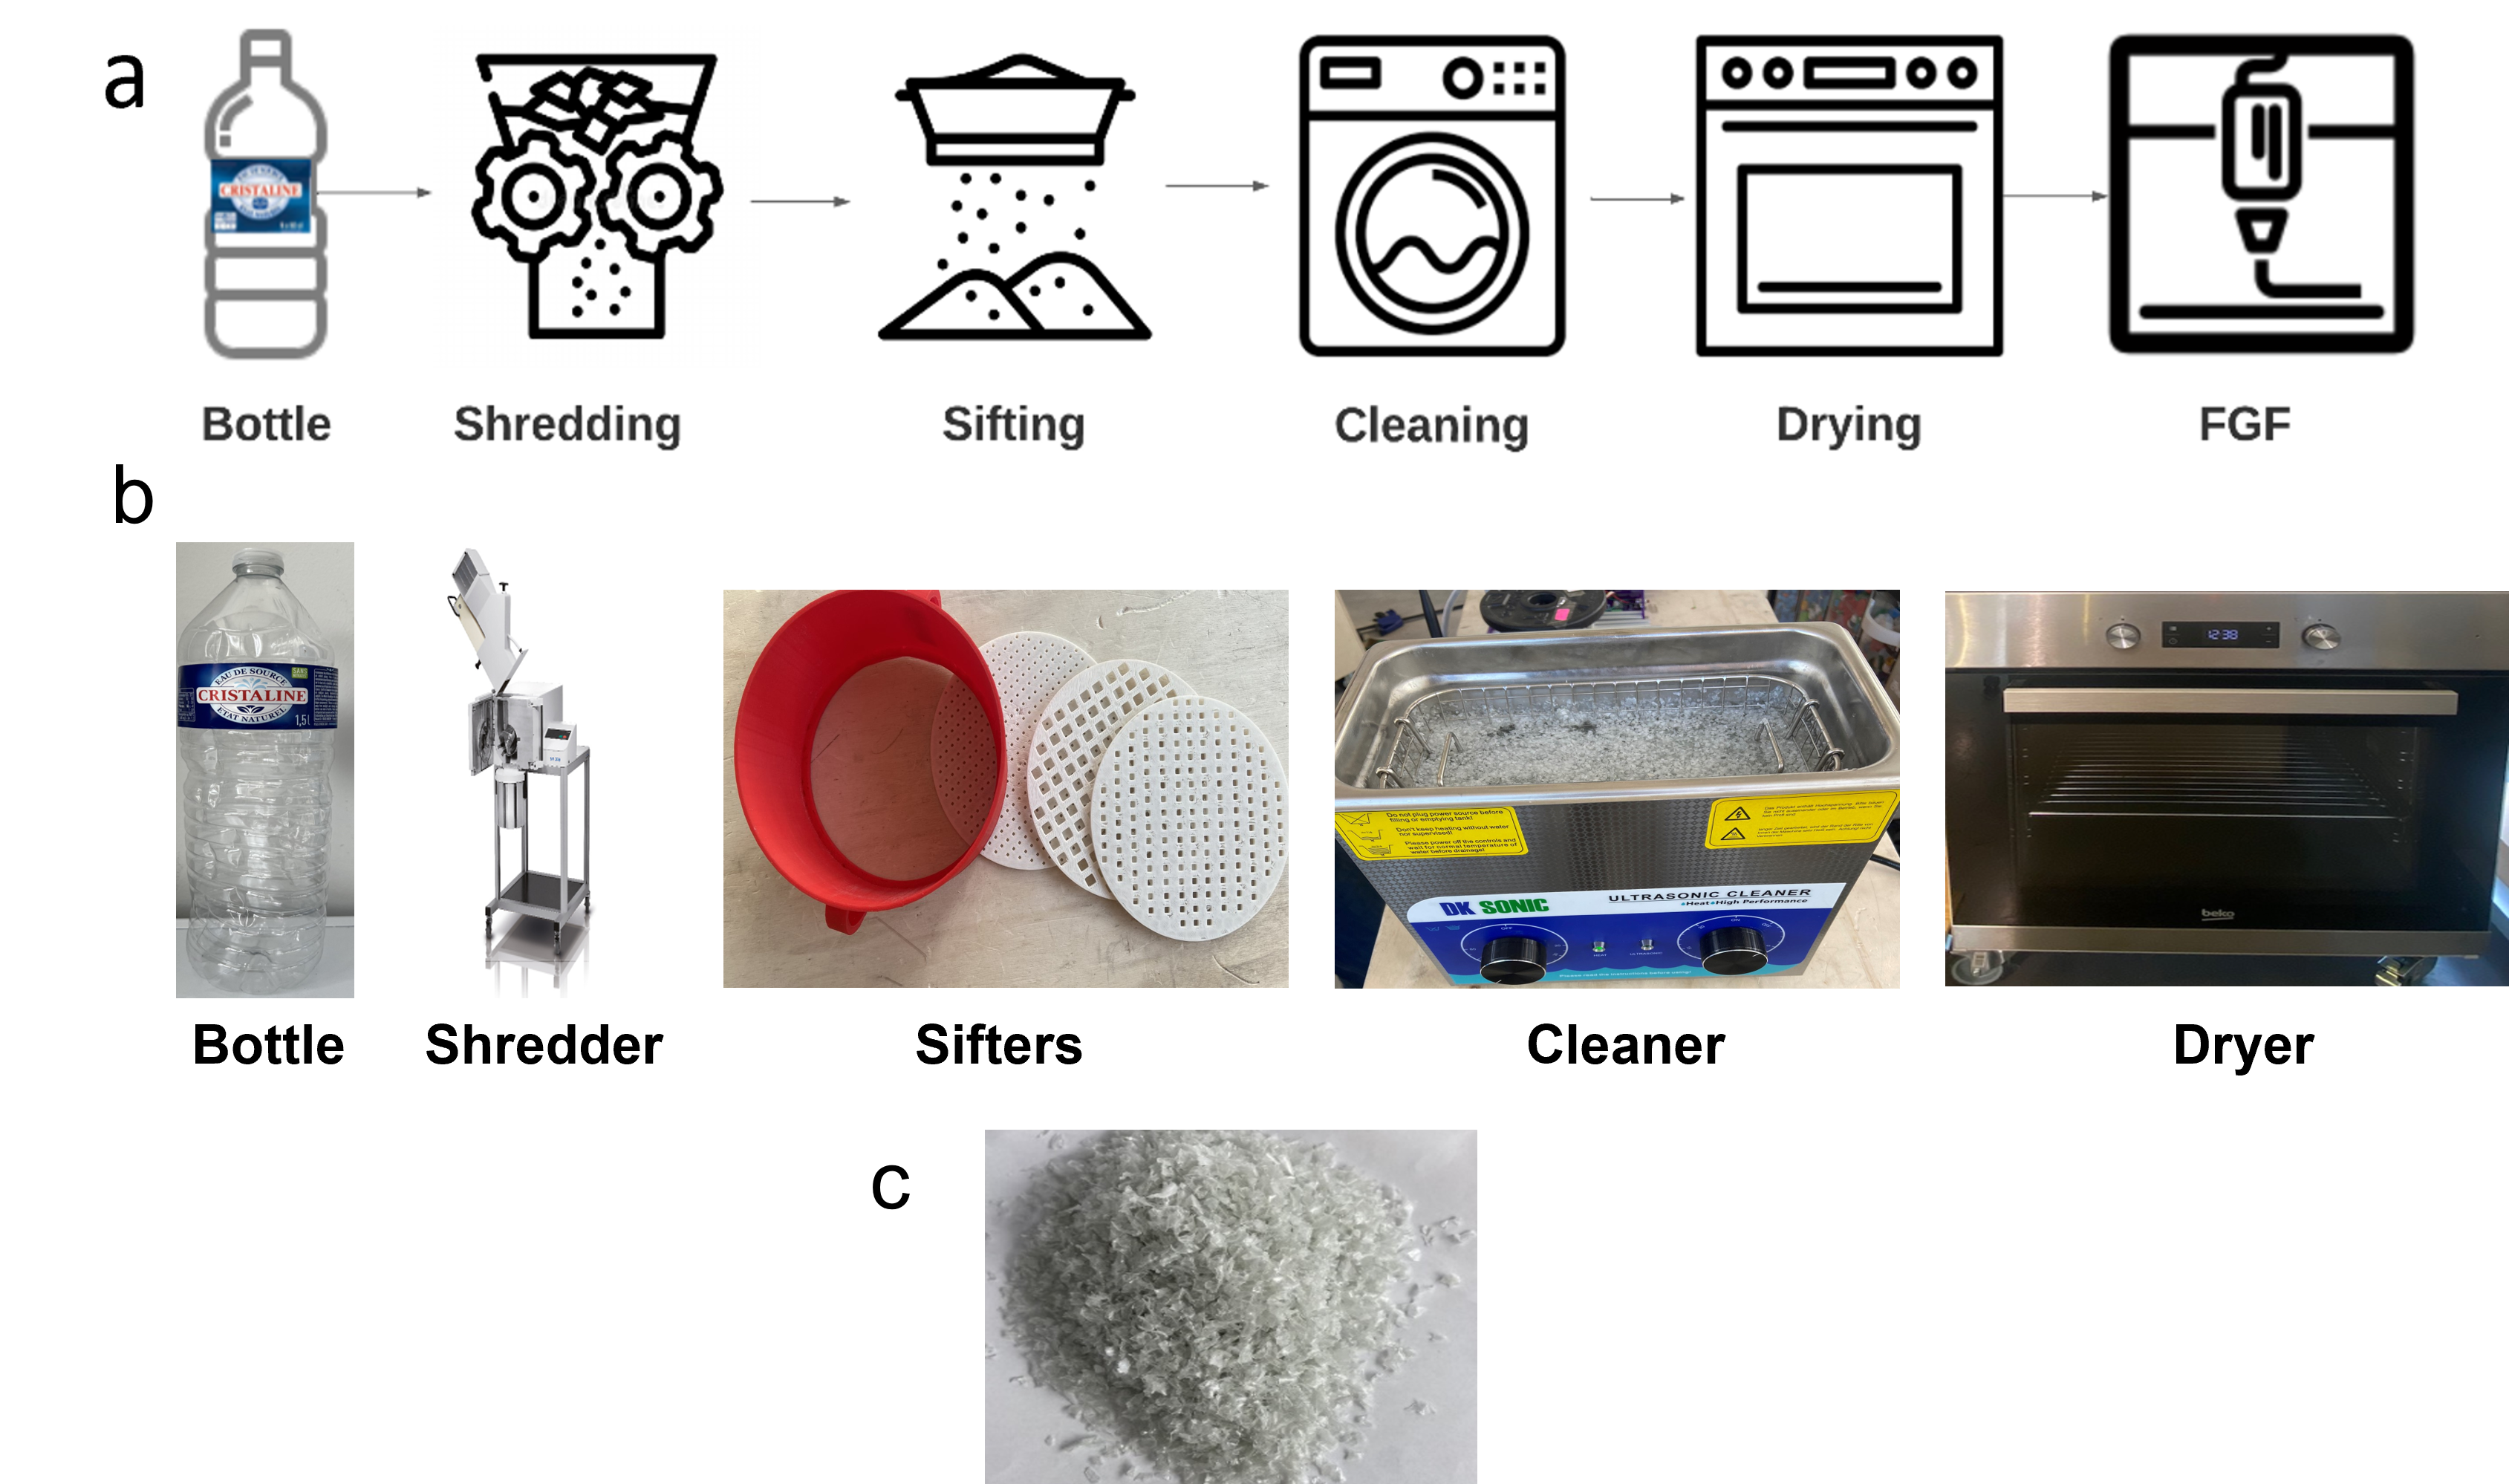
\includegraphics{figures/Fig_2.png}

}

\caption{\label{fig-fig1}Process steps to prepare the collected
material}

\end{figure}

The material composition was calculated as a function of the mass of the
bottles and caps separately. The percentage (\%) of bottle-cap was found
to be \textasciitilde90\%rPET (bottle) and \textasciitilde10\% rHDPE
(cap). The complete bottle was shredded without separation of both
materials thus this percentage is constant for all the samples.

\hypertarget{material-preparation-and-characterization}{%
\subsection{Material preparation and
characterization}\label{material-preparation-and-characterization}}

\hypertarget{material-particle-size-analysis--granulometry-}{%
\subsubsection{Material particle size analysis
-Granulometry-}\label{material-particle-size-analysis--granulometry-}}

In order to ensure the particle size suitable for printing, the
granulate particles were characterized using the open-source ImageJ
software {[}@imagej2023{]}. The size characteristics of the particles
were evaluated in four different samples: vPET (used as a reference) and
the raw material sifted into three different sizes: \(1.5~mm\),
\(3~mm\), and \(5~mm\).

\hypertarget{fourier-transform-infrared-spectroscopy-ftir-}{%
\subsubsection{Fourier-transform infrared spectroscopy
--FTIR-}\label{fourier-transform-infrared-spectroscopy-ftir-}}

FTIR spectroscopy was conducted to determine the composition of the
bottle and identify any impurities, plasticizers, or additives. The
analysis involving testing separate samples of rPET and rHDPE.
Additionally, a printed sample of both materials was examined to
identify any potential chemical bonding. Each sample was measured at two
different points, with three measurements taken at each point. The
resulting curves were then normalized and analyzed using Origin Pro 8.
The Fourier transform infrared spectra were recorded in the range of
\(4000~cm^{-1}\) to \(375~cm^{-1}\) with a resolution of \(4~cm^{-1}\)
using a Bruker IFS 66V spectrophotometer.

\hypertarget{differential-scanning-calorimetry-dsc-}{%
\subsubsection{Differential scanning calorimetry
--DSC-}\label{differential-scanning-calorimetry-dsc-}}

Differential scanning calorimetry analysis was performed using a DSC-1
Mettler Toledo with STARe software operating under nitrogen atmosphere
at heating rate and cooling rate of \(10~°C/min\). The samples
investigated were rPET, rHDPE, and rPET90//rHDPE10. Three cycles were
conducted: the first involved heating from 20°C to 270°C, cooling to
20°C and reheating to 270°C. The rHDPE sample was analyzed using similar
cycles but with the maximum temperature set at 250°C and the blend was
tested at temperatures ranging from -20 to 270°C. The glass transition
temperature (Tg) of rPET was determined during the first heating cycle,
while the Tg of rPET90//rHDPE10 was determined during the second heating
cycle, along with the melting point of all materials. The
crystallization temperature (Tc) was determined during the cooling cycle
for each material. The degree of crystallinity (Xc) was calculated from
the second cycle for recycled materials and the first cycle for the
blend, as expressed in equation (1) {[}@taghavi2018; @pan2020{]}:

\begin{equation}\protect\hypertarget{eq-dsc}{}{
X_{c}(\%) = \frac{\Delta H_{m}}{w \cdot \Delta H_{m}^\circ}
}\label{eq-dsc}\end{equation}

Where, \(\Delta H_{m}\) is the latent heat of melt, \(w\) is the weight
percentage of polymer in the blend, and \(\Delta H_{m}^\circ\) is the
reference heat of 100\% crystalline PET (\(140~J/g\)) and HDPE
(\(293~J/g\)), respectively, provided in the literature {[}@pan2020;
@kratofil2006{]}.

\hypertarget{melt-flow-index-mfi-}{%
\subsubsection{Melt Flow Index --MFI-}\label{melt-flow-index-mfi-}}

The melt-flow index (MFI) of rPET90//rHDPE10 flakes was determined using
an Instron CEAST MF20. The analysis was performed using three samples of
\textasciitilde5 g at a temperature of 255 °C with a 2.16 kg weight
following the ASTM D1238 standard. The process was repeated three times.
The average value of the three results was reported in units of
\(gr/10 \times min\).

\hypertarget{density}{%
\subsubsection{Density}\label{density}}

The material's density was calculated as follows: first, the volume was
found by measuring the dimensions of a solid \(50x50x50~mm\) cubic
geometry fabricated by injecting rPET90//rHDPE10 flakes into a square
mold with a known volume using an open-source desktop injection
machine(Holipress, Holimaker, France). Then, the model was weighed, and
the mass was obtained. Finally, the density was calculated as expressed
in Equation~\ref{eq-density}. To ensure the accuracy of the test it was
performed twice and the average value was reported in \(g/cm^{3}\).

\begin{equation}\protect\hypertarget{eq-density}{}{
\rho = V/m    \qquad \left[ \frac{g}{cm^{3}} \right]
}\label{eq-density}\end{equation}

Where, \(\rho\) is the density, \(V\) is the volume, and \(m\) the mass.

Afterwards, experimental results were compared with the theoretical
blend density which could be calculated by
Equation~\ref{eq-density_theory}.

\begin{equation}\protect\hypertarget{eq-density_theory}{}{
\rho_{12}= \frac{1}{\frac{W_{1}}{\rho_{2}} + \frac{W_{2}}{\rho_{2}}} \qquad \left[ \frac{g}{cm^{3}} \right]                                               
}\label{eq-density_theory}\end{equation}

Where, \(\rho_{12}\) is the density of the blend, \(W_{1}\) and
\(W_{2}\), the weight fractions of each polymer, \(\rho_{1}\) and
\(\rho_{2}\), the theoretical density of each polymer for PET
(\(~1.38~g/cm^{3}\)) and HDPE 0.93 to 0.97 \(g/cm^{3}\)
{[}@jonathanguidigo12017{]}.

\hypertarget{printing-process}{%
\subsection{Printing process}\label{printing-process}}

\hypertarget{establishing-optimal-parameters}{%
\subsubsection{Establishing optimal
parameters}\label{establishing-optimal-parameters}}

Establishing the optimal combinations of parameters is essential for
improve the quality and mechanical properties of printed parts
{[}@jaisinghsheoran2020{]}. According to @oberloier2022, particle swarm
optimization (PSO) is an accurate and time-effective method for achiving
this goal. To optimize the 3-D printing parameters for the
rPET90//rHDPE10 material in the GigabotX we utilized the open-source PSO
Experimenter platform which is available for Linux. The methodology
developed by @oberloier2022 was followed during the optimization. For
benchmarking purposes, three artifacts were printed: a line, a plane,
and a cube. These artifacts were modeled in CAD software Onshape CAD
v1.150 and sliced using Prusaslicer v2.52.0. Figure~\ref{fig-cad}
presents the geometry models and dimensions of the artifacts.

\begin{figure}

{\centering 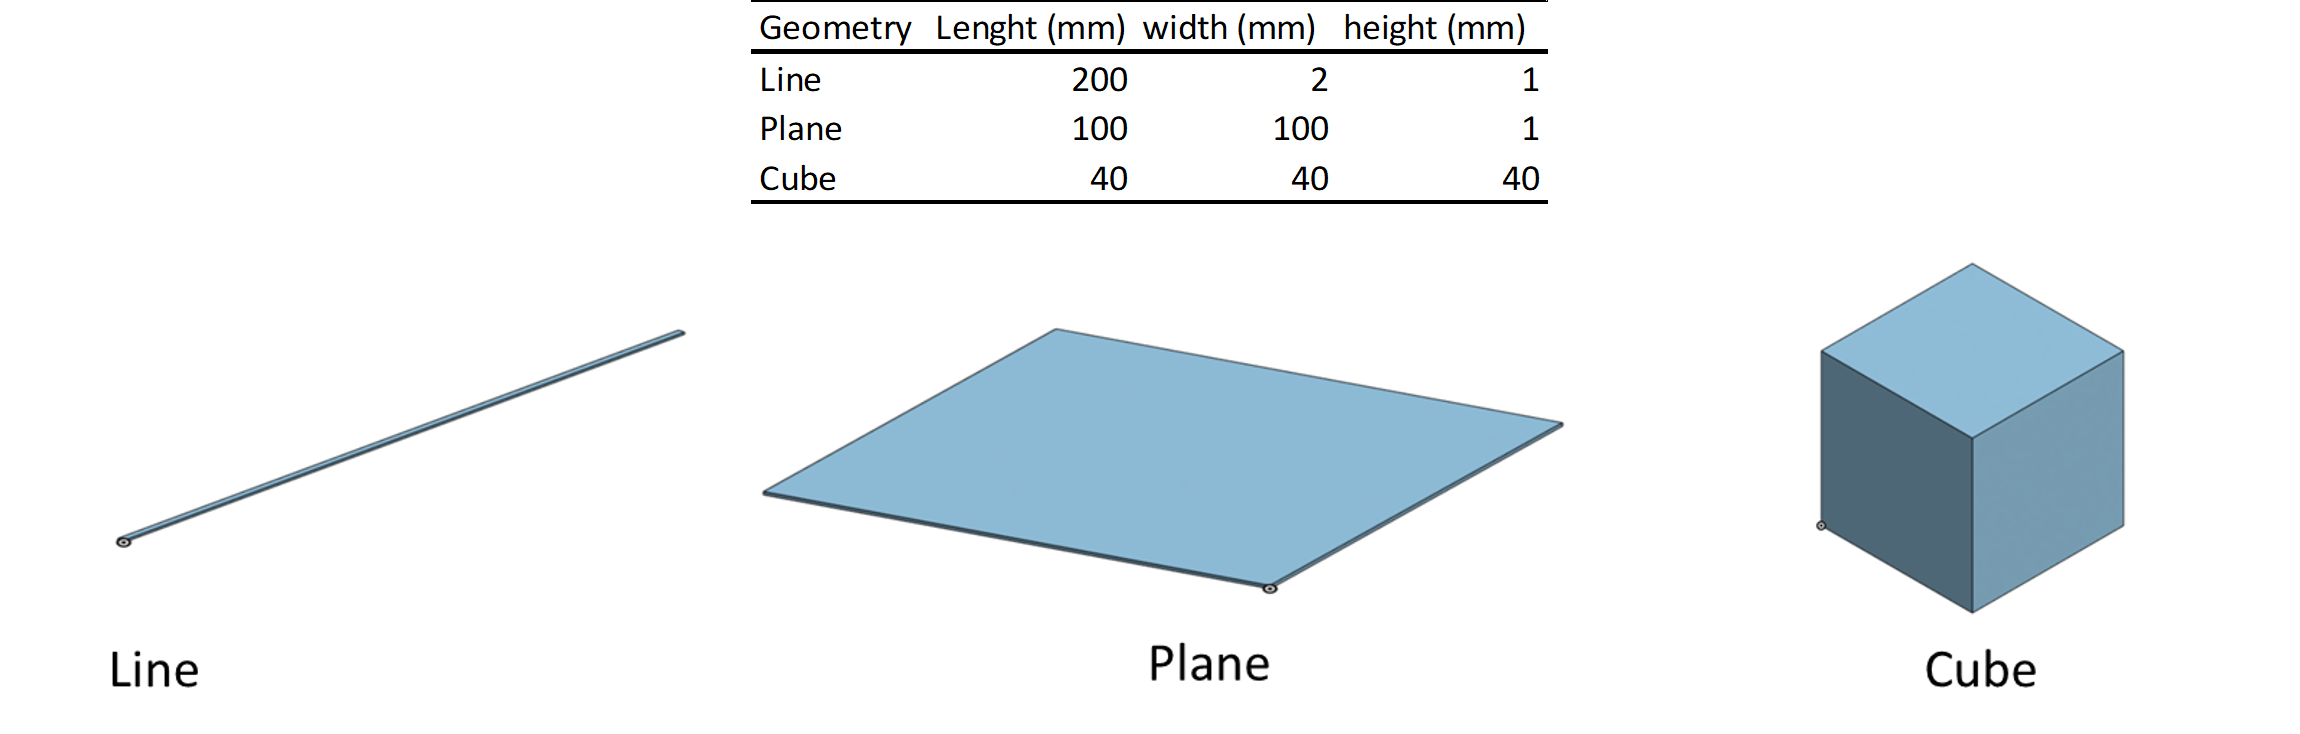
\includegraphics{figures/Figure-2.png}

}

\caption{\label{fig-cad}Dimensions and CAD models of the geometries used
for parameters optimization.}

\end{figure}

Four parameters were assessed: 1) nozzle temperature, 2) bed
temperature, 3) printing speed and 4) extrusion multiplier
{[}@oberloier2022a{]}. The initial parameters for the line are presented
in Table 1a while additional parameters were obtained from preliminary
experimental work shown in Table 1.b. Finally, the PSO tuning parameters
were found in the previous PSO work {[}@oberloier2022{]} Table 1.c.

\begin{table}

\caption{\label{tbl-table1}table 1}\begin{minipage}[t]{\linewidth}
\subcaption{\label{tbl-table1-1}Line optimization initial parameters }

{\centering 

\tabularnewline

\centering\begingroup\fontsize{12}{14}\selectfont

\begin{tabular}{llrrll}
\toprule
Variable & Min & Max & Guess & True/False & Description\\
\midrule
\cellcolor{gray!6}{T1} & \cellcolor{gray!6}{255} & \cellcolor{gray!6}{270} & \cellcolor{gray!6}{260} & \cellcolor{gray!6}{TRUE} & \cellcolor{gray!6}{Temperature Zone 1 on GigabotX}\\
Tb & 80 & 90 & 85 & TRUE & Bed temperature\\
\cellcolor{gray!6}{Ps} & \cellcolor{gray!6}{10} & \cellcolor{gray!6}{25} & \cellcolor{gray!6}{15} & \cellcolor{gray!6}{TRUE} & \cellcolor{gray!6}{Printing Speed}\\
E & 0.5 & 2 & 1 & FALSE & Extrusion Multiplier\\
\bottomrule
\end{tabular}
\endgroup{}

}

\end{minipage}%
\newline
\begin{minipage}[t]{0.50\linewidth}
\subcaption{\label{tbl-table1-2}Fixed parameters to perform printing parameters optimization based on
PSO }

{\centering 

\tabularnewline

\centering\begingroup\fontsize{11}{13}\selectfont

\begin{tabular}{lll}
\toprule
Parameters & Value & Units\\
\midrule
\cellcolor{gray!6}{Layer height} & \cellcolor{gray!6}{0.5} & \cellcolor{gray!6}{mm}\\
Width & 2 & mm\\
\cellcolor{gray!6}{T2} & \cellcolor{gray!6}{230} & \cellcolor{gray!6}{°C}\\
T3 & 220 & °C\\
\cellcolor{gray!6}{Cooling} & \cellcolor{gray!6}{0} & \cellcolor{gray!6}{\%}\\
\addlinespace
Infill density & 2 & \%\\
\bottomrule
\end{tabular}
\endgroup{}

}

\end{minipage}%
%
\begin{minipage}[t]{0.05\linewidth}

{\centering 

~

}

\end{minipage}%
%
\begin{minipage}[t]{0.45\linewidth}
\subcaption{\label{tbl-table1-3}Recommended parameters for PSO tuning }

{\centering 

\tabularnewline

\centering\begingroup\fontsize{11}{13}\selectfont

\begin{tabular}{lr>{\raggedright\arraybackslash}p{4cm}}
\toprule
Variable & Value & Description\\
\midrule
\cellcolor{gray!6}{Kv} & \cellcolor{gray!6}{0.5} & \cellcolor{gray!6}{The emphasis given to the velocity component}\\
Kp & 1.0 & The emphasis given to a particle's personal best position\\
\cellcolor{gray!6}{Kg} & \cellcolor{gray!6}{2.0} & \cellcolor{gray!6}{The emphasis given to the swarm's group's best position}\\
\bottomrule
\end{tabular}
\endgroup{}

}

\end{minipage}%

\end{table}

\hypertarget{fused-granular-fabrication-fgf-}{%
\subsubsection{Fused Granular Fabrication
--FGF-}\label{fused-granular-fabrication-fgf-}}

To print the obtained raw material, a modified open-source printer with
three heat zones (Gigabot XL re:3D, Houston, TX, USA) was utilized as
illustrated in Figure~\ref{fig-gigabot}. The machine is a single screw
extrusion-based 3-D printer capable of direct printing pellets, flakes,
or granules, with a nozzle size of \(1.75~mm\). For this study, a chair
was printed to evaluate the material's ability to be 3-D printed and the
printer's capability to produce large objectslike furniture. The ideal
parameters determined for the cube geometry were employed to print the
final part.

\begin{figure}

{\centering 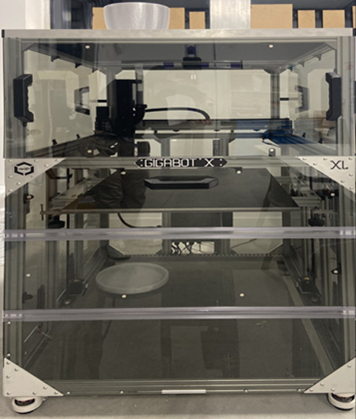
\includegraphics{figures/Figure_4_Giga.png}

}

\caption{\label{fig-gigabot}Fused granular fabrication printer Gigabot}

\end{figure}

\hypertarget{results-and-discussion}{%
\section{Results and discussion}\label{results-and-discussion}}

\hypertarget{material-characterization}{%
\subsection{Material characterization}\label{material-characterization}}

Both the polymeric components of the bottle and the blend were
characterized and analyzed to determine their properties using different
methods as described in the preceding section.

\hypertarget{material-particle-size-analysis-granulometry}{%
\subsubsection{Material particle size analysis
(granulometry)}\label{material-particle-size-analysis-granulometry}}

Previous studies demonstrated that particles with areas smaller than
\(22~mm^{2}\) were optimal for printing without experiencing jamming or
under-extrusion problems {[}@woern2018{]}. However, our experiments
revealed that particles with areas exceeding \(10~mm^{2}\) caused
clogging in the feeding system and auger screw of the machine. As a
result, granulometry analysis was performed using three different mesh
sizes.

\begin{figure}

\begin{minipage}[t]{0.57\linewidth}

{\centering 

\raisebox{-\height}{

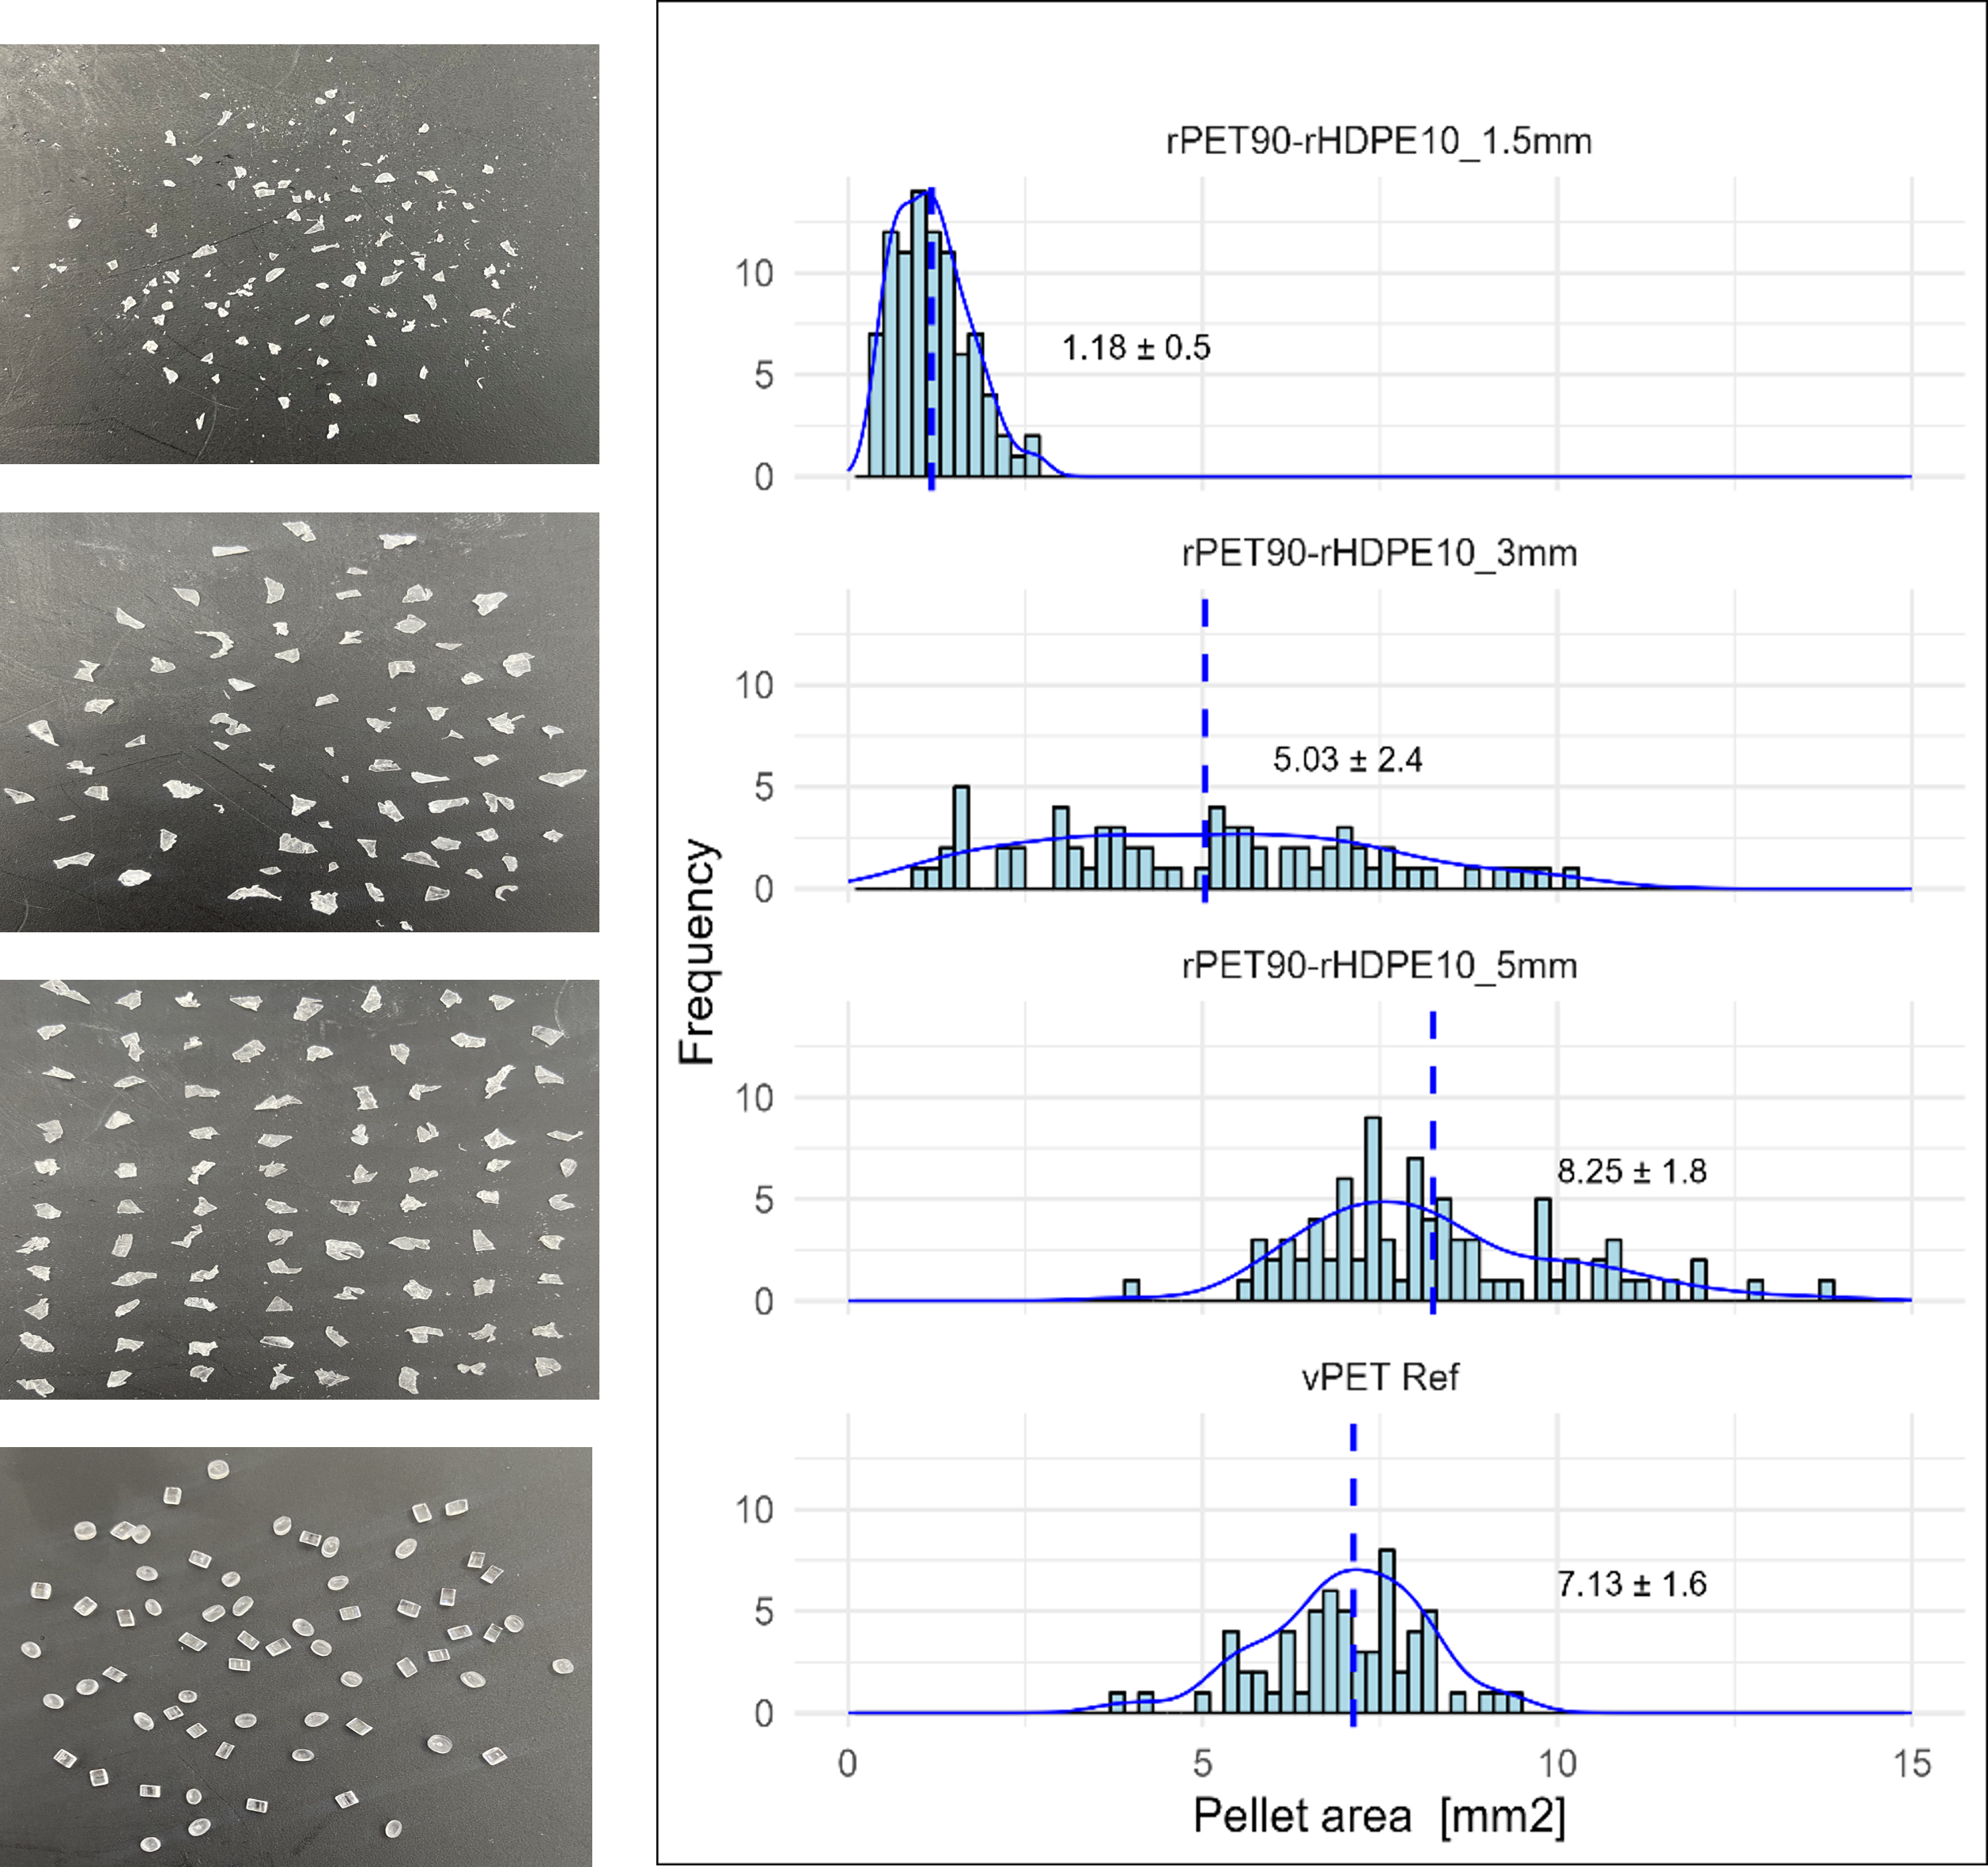
\includegraphics{figures/Figure_5_granulometry.png}

}

\caption{\label{fig-granulometry}Granulometry analysis}

}

\end{minipage}%
%
\begin{minipage}[t]{0.03\linewidth}

{\centering 

~

}

\end{minipage}%
%
\begin{minipage}[t]{0.40\linewidth}

{\centering 

\raisebox{-\height}{

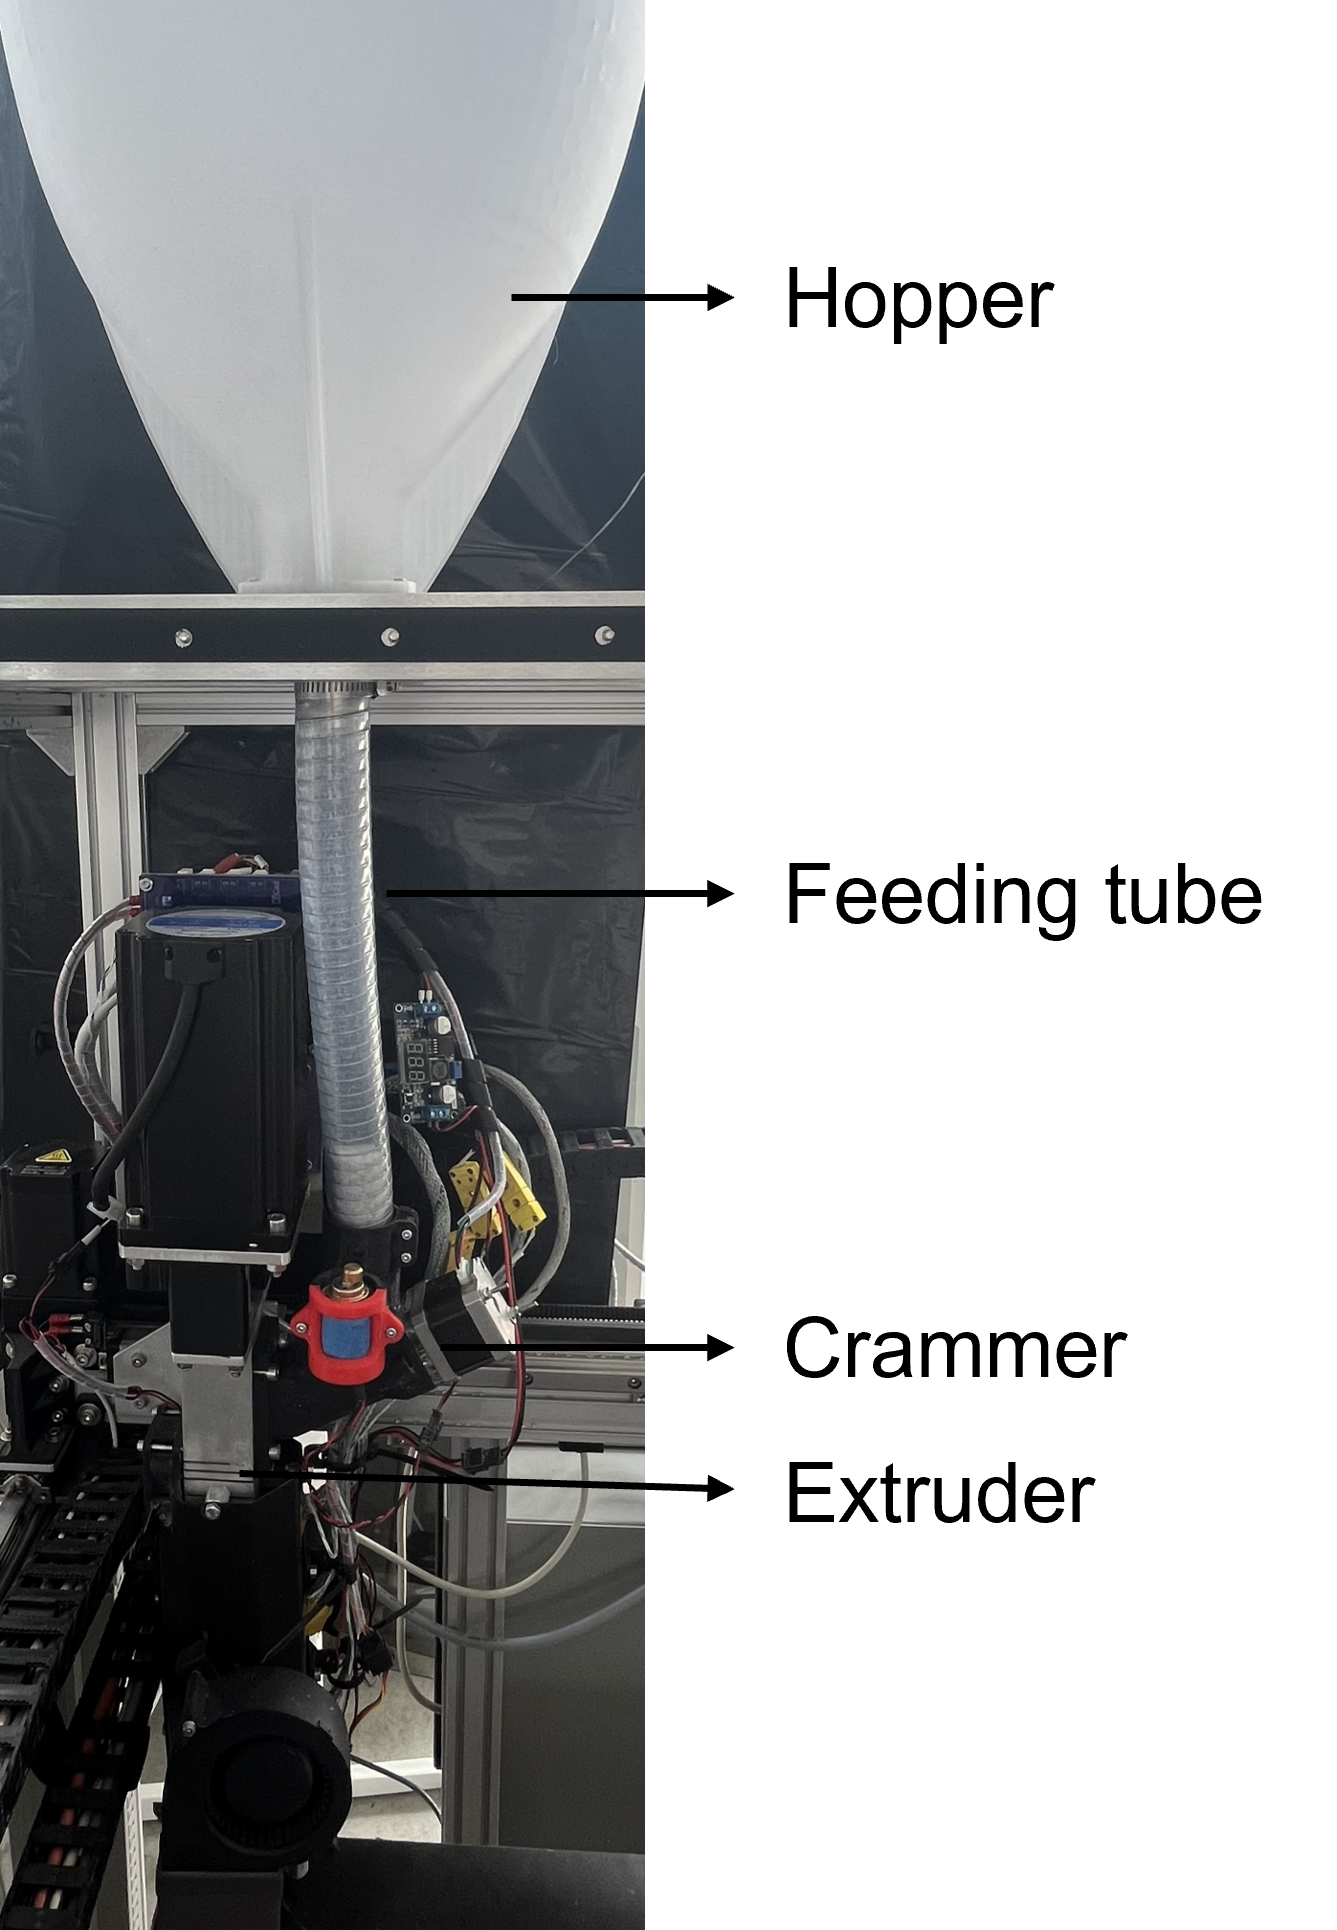
\includegraphics{figures/Figure_6_crammer.png}

}

\caption{\label{fig-crammer}Gigabot feeding system}

}

\end{minipage}%

\end{figure}

Figure~\ref{fig-granulometry} presents the obtained results, indicating
that particles sifted at \(5~mm\) exhibited an average area similar to
the reference. There are, however, particles with areas exceeding
\(9~mm^{2}\) caused blockages in the feeding and extrusion section.
Particles sifted to \(1.5~mm\) displayed a distribution ranging from 0
to approximately \(3~mm^{2}\), which was deemed too small for printing
purposes. The presence of these small particles can lead to their
complete melting in the initial heat zone, thereby impeding the smooth
flow of other particles and preventing the necessary pressure for
extruding the melted particles further down the screw. Although flakes
measuring 3 mm exhibited a more dispersed distribution and slightly
smaller area compared to the reference, they were found to be optimal
for printing.

The final objects, however, still showed under-extrusion issues. To
address this problem, a crammer was implemented {[}@little2020{]} as
presented in Figure~\ref{fig-crammer}. The crammer physically pushes
particles towards the auger, facilitating their transfer from the
feeding tube to the extruder. After the crammer implementation the
under-extrusion issues were greatly reduced. It was concluded that
flakes with areas ranging from \(1.5~mm^{2}\) to \(10~mm^{2}\) were the
most suitable for printing when using a crammer to assist the feeding
system.

\hypertarget{chemical-analysis-from-ftir}{%
\subsubsection{Chemical analysis from
FTIR}\label{chemical-analysis-from-ftir}}

Chemical structure information of the materials was obtained using FTIR
spectroscopy, which allowed the analysis of the characteristic spectral
bands of the polymers.

In the case of rPET (bottle) four distinct bands can be observed in
Figure~\ref{fig-FTIR}. The first band, located at \(1713 cm^{-1}\)
represent the \(C=O\) double bond. The second band, at \(1240 cm^{-1}\),
corresponds to the \(C-O\) single bond ester. The third band, at
\(1093 cm^{-1}\), is associated with band the methylene group and
vibrations of the ester bond. Lastly, a band at \(722 cm^{-1}\) which
represents the CH2 rocking bending vibration. Similar results were
reported in the literature for PET derived from recycled water bottles,
soda bottles, and food containers {[}@zander2018{]}.

Regarding rHDPE (caps), four characteristic peaks were identified: the
C-H functional group bond at \(2915cm^{-1}\) and \(2847~cm^{-1}\), the
primary bending mode of the -CH2 at \(1465~cm^{-1}\) and the CH2 rocking
bending vibration at \(729 ~cm^{-1}\). The results obtained confirmed
the chemical structures of the starting materials. Additionally, no
other indicative resonances, apart from those associated with the
polymer structures were detected. This leads to the conclusion that
there were no significant amounts of additives or plasticizers present
in either of the samples. Moreover, the spectrum of the printed blend
(rPET90//rHDPE10) exhibited identical characteristic peaks to those
observed in the bottle, thus confirming the predominant presence of PET.
There are, however, noticeable differences between \(1000 ~cm^{-1}\) and
\(720 ~cm^{-1}\) as well as in the C-H bond (\(2915~cm^{-1}\) and
\(2847 ~cm^{-1}\) peaks), which confirm the presence of HDPE (cap). The
observed shift can be attributed to interactions between the two
materials.

\begin{figure}

{\centering 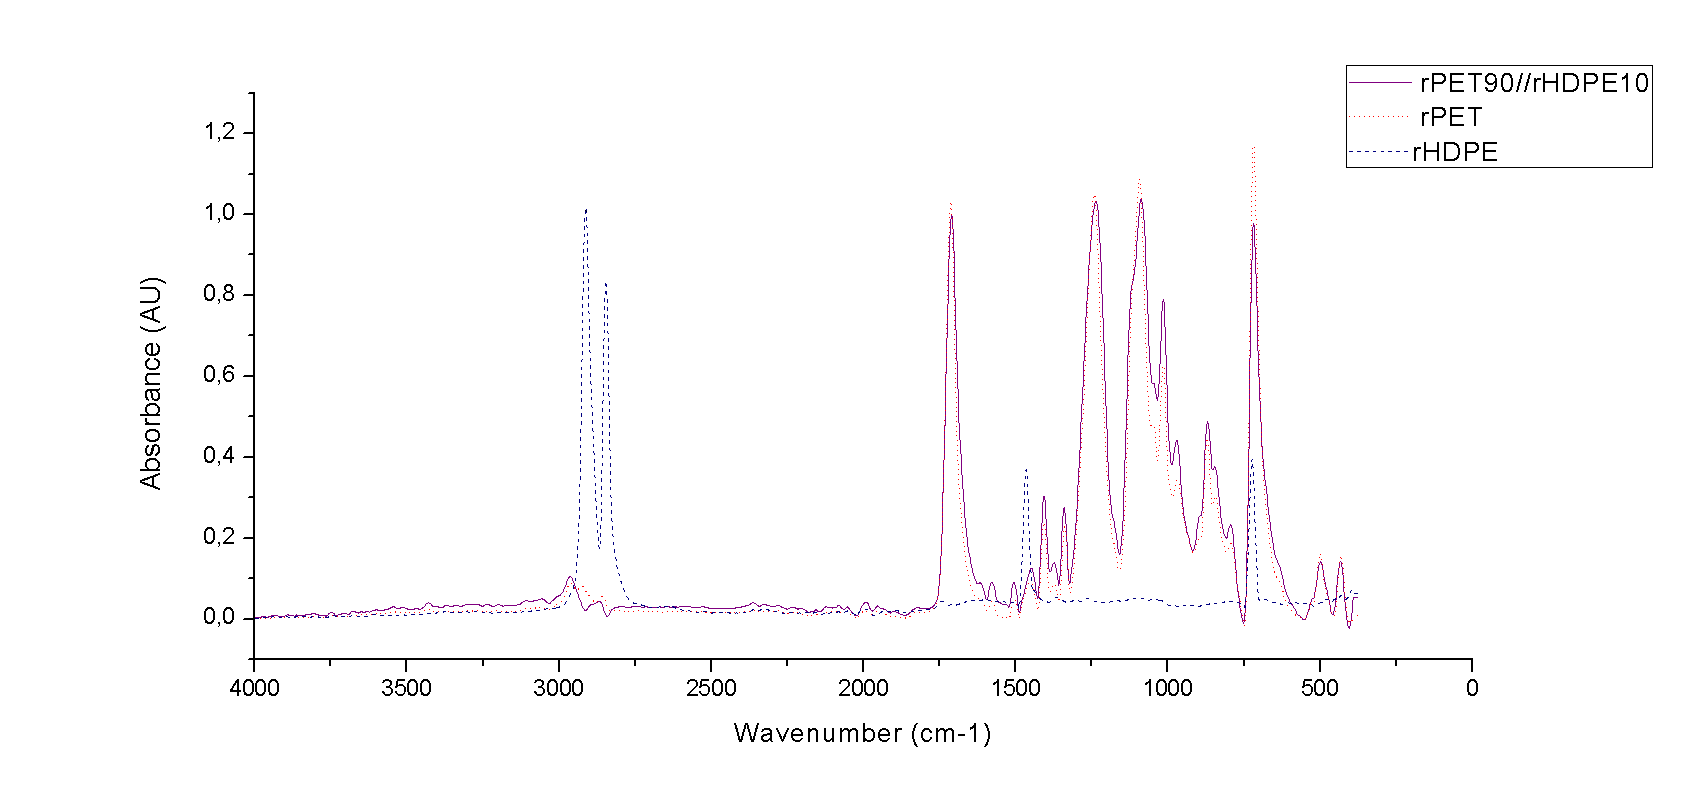
\includegraphics[width=0.9\textwidth,height=\textheight]{figures/Figure_7_FTIR.png}

}

\caption{\label{fig-FTIR}FTIR spectra of rPET, rHDPE, and their blend}

\end{figure}

\hypertarget{thermal-analysis-dsc}{%
\subsubsection{Thermal analysis DSC}\label{thermal-analysis-dsc}}

The thermal properties of both recycled materials and their blend were
characterized using DSC to establish a baseline for optimizing process
parameters of 3-D printing.

Two distinct endothermic peaks are observed in the representative
heating and cooling thermograms shown in Figure~\ref{fig-DCS}, for the
printed blend sample. These peaks are associated with the fusion of the
crystalline fractions of rHDPE and rPET, providing confirmation of the
immiscibility of both materials. Moreover, the enthalpy of fusion and
crystallization of the rHDPE in the blend is significantly reduced,
which can be attributed to the low percentage of HDPE present in the
blend. Furthermore, the presence of a cold crystallization peak in the
blend, but not in the individual polymers,suggests an interaction
between the two polymers. It is possible that the rHDPE acts as a
nucleating agent in this interaction. Table 2.lists the thermal
properties of rPET, rHDPE and rPET90//rHDPE10. The melting points of
rHDPE and rPET are 131.7 °C and 249.9 °C, respectively, which align with
previous findings in the literature {[}@vaucher2022; @lei2009;
@chen2015{]}. It is observed that the melting and crystallization
temperature of rPET increased, while that of rHDPE slightly decreased.
Furthermore, the crystallization of rPET was found to be somewhat
affected by the presence of rHDPE, resulting in a 3.5\% increase in
degree of crystallization.This can be attributed to the rHDPE acting as
a germination point for crystallization {[}@vaucher2022{]}. The slight
changesin the fusion-crystallization temperatures and degree of
crystallinity of rPET indicate an interaction of both polymers.

\begin{figure}

\begin{minipage}[t]{\linewidth}

{\centering 

\raisebox{-\height}{

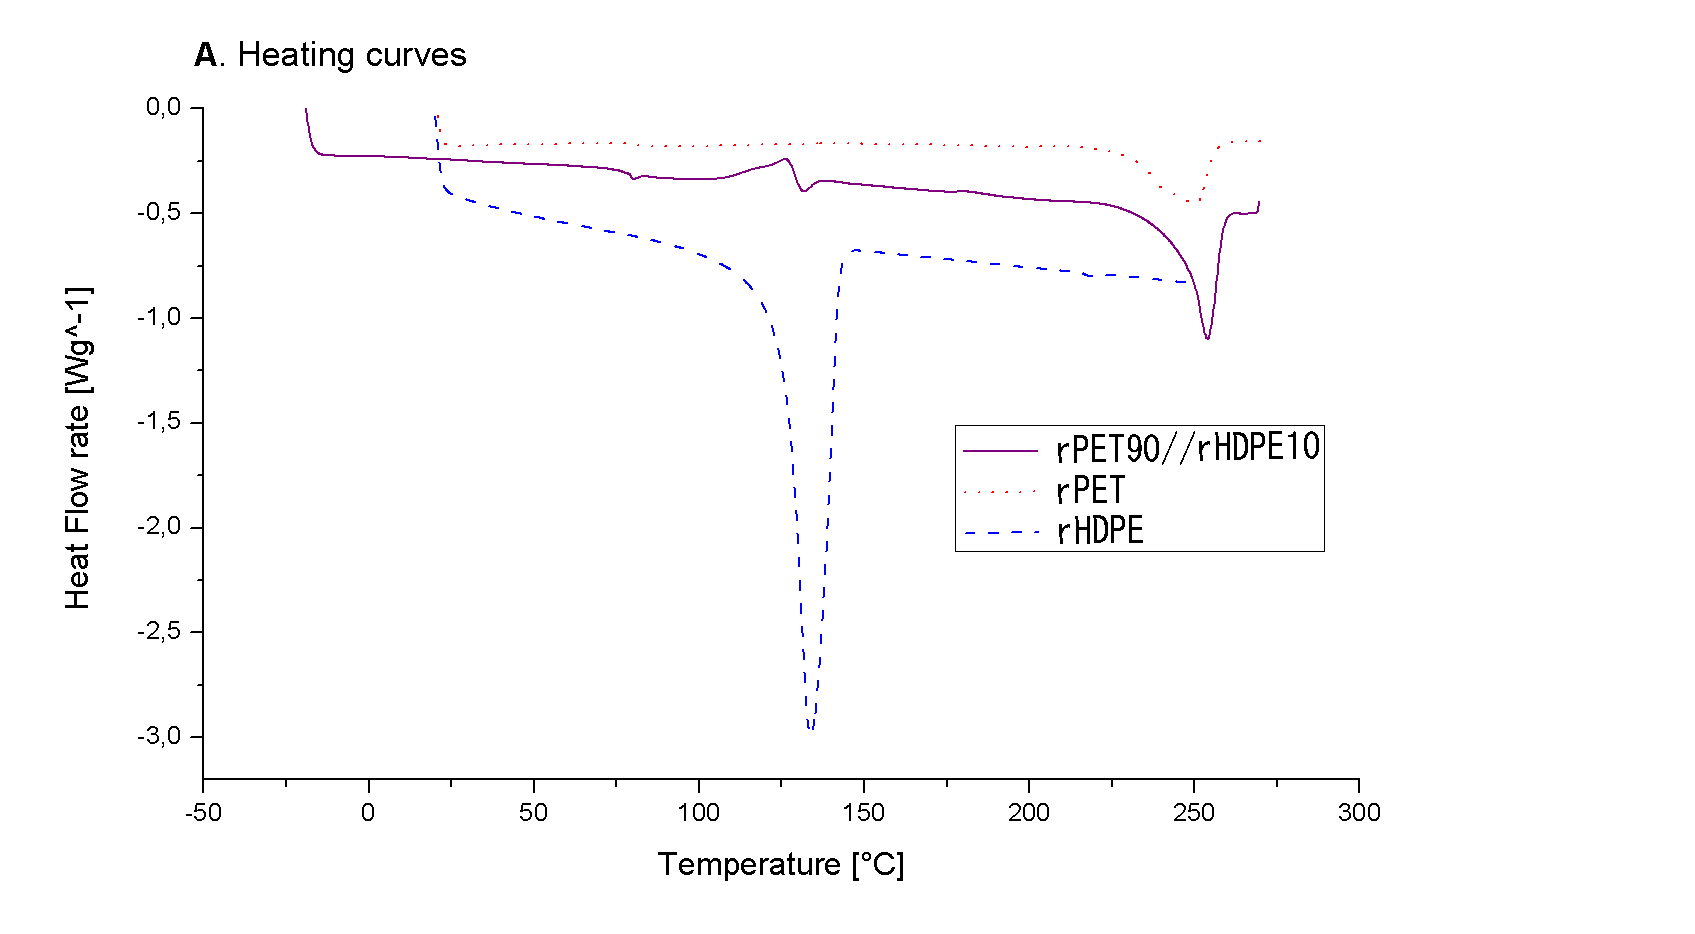
\includegraphics{figures/Figure_8a_DSC.png}

}

}

\subcaption{\label{fig-DCSa}Heating curves}
\end{minipage}%
\newline
\begin{minipage}[t]{\linewidth}

{\centering 

\raisebox{-\height}{

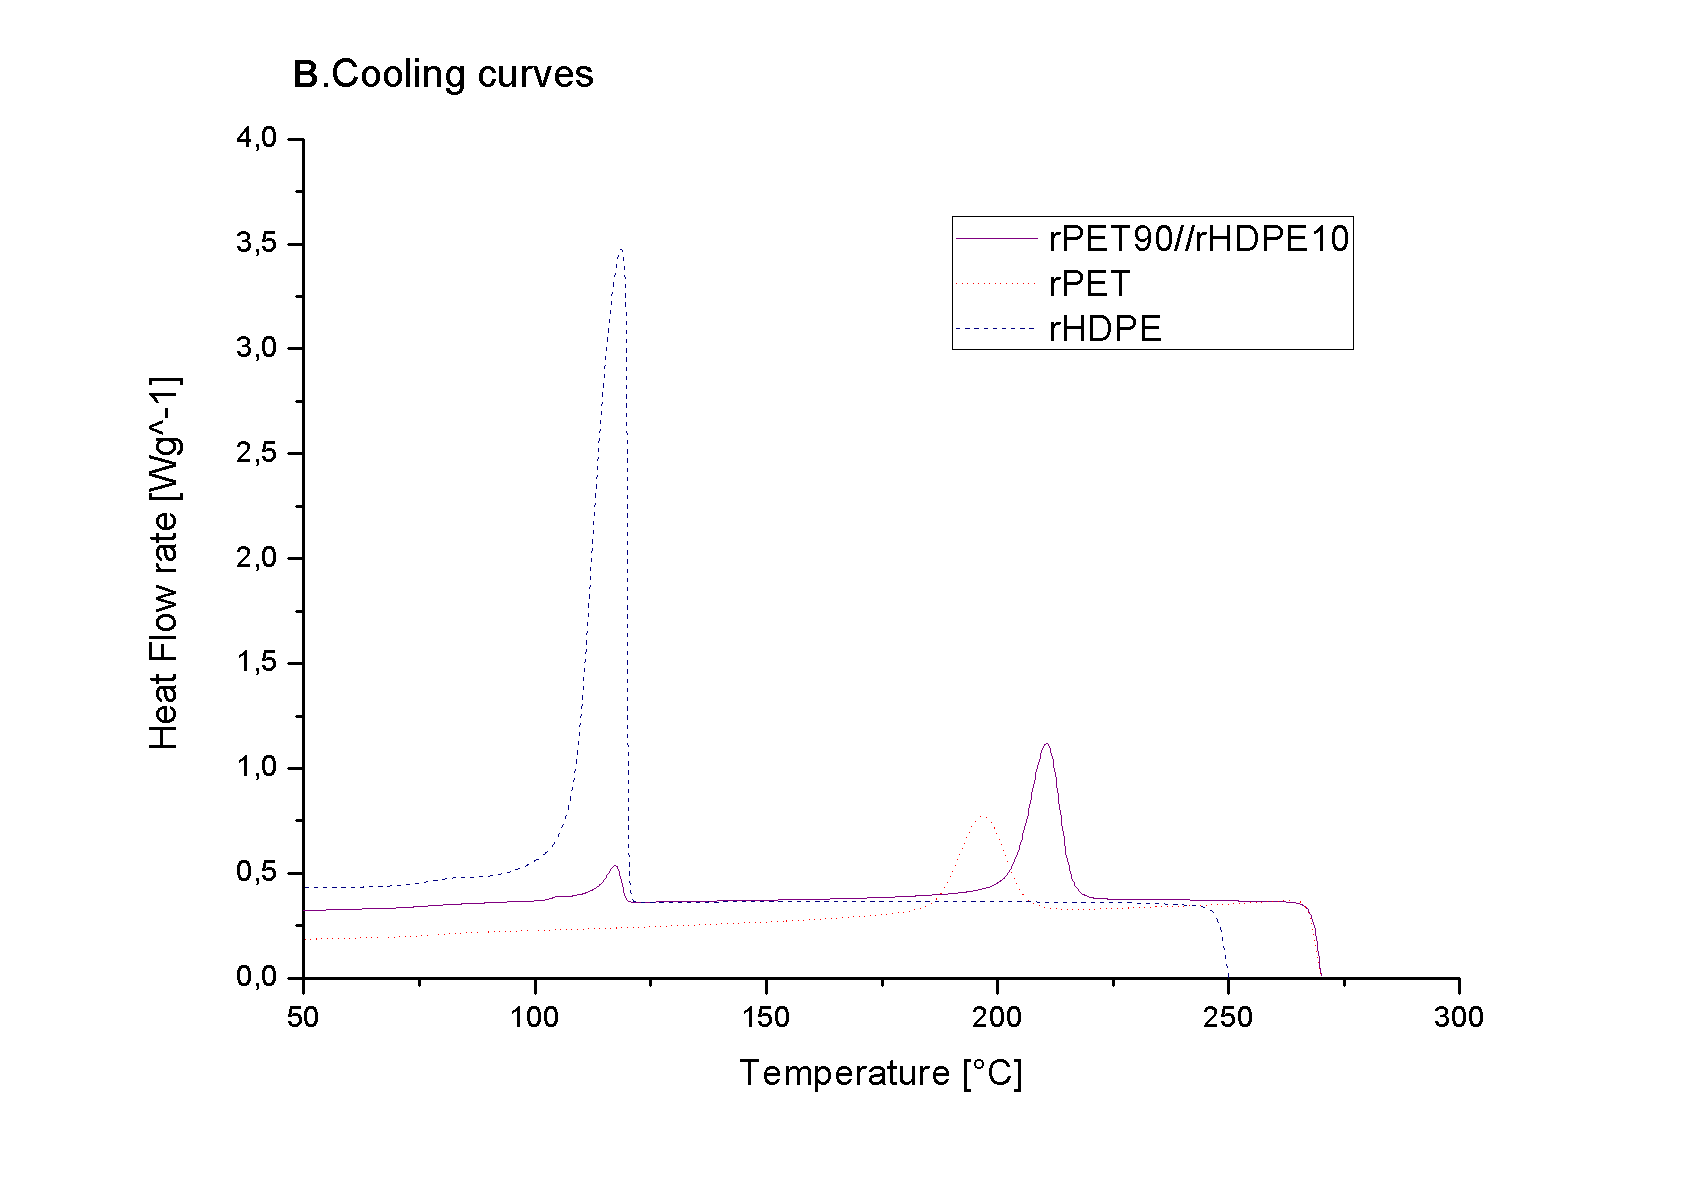
\includegraphics{figures/Figure_8b_DSC.png}

}

}

\subcaption{\label{fig-DCSb}Cooling curve}
\end{minipage}%

\caption{\label{fig-DCS}DSC thermograms of recycled materials and
blends}

\end{figure}

\begin{table}
\caption{Thermal analysis of rPET, rHDPE, and their blend}\tabularnewline

\centering\begingroup\fontsize{8}{10}\selectfont

\begin{tabular}[t]{llllllll}
\toprule
\multicolumn{1}{c}{ } & \multicolumn{1}{c}{Glass transition} & \multicolumn{2}{c}{Melting} & \multicolumn{3}{c}{Crystallization } & \multicolumn{1}{c}{\% Crystallinity} \\
\cmidrule(l{3pt}r{3pt}){2-2} \cmidrule(l{3pt}r{3pt}){3-4} \cmidrule(l{3pt}r{3pt}){5-7} \cmidrule(l{3pt}r{3pt}){8-8}
Sample & Tg (°C) & Tm  (°C ) & ΔHm (J/g) & Tc  (°C ) & ΔHc (J/g) & ΔHcc (J/g) & Xc\\
\midrule
\cellcolor{gray!6}{rPET} & \cellcolor{gray!6}{82} & \cellcolor{gray!6}{249.9} & \cellcolor{gray!6}{32.3} & \cellcolor{gray!6}{196.7} & \cellcolor{gray!6}{33.3} & \cellcolor{gray!6}{-} & \cellcolor{gray!6}{23.1}\\
rHDPE & - & 133.8 & 172 & 118.7 & 158.2 & - & 58.7\\
\cellcolor{gray!6}{rPET90/rHDPE10} & \cellcolor{gray!6}{77 / -} & \cellcolor{gray!6}{254/131.7} & \cellcolor{gray!6}{40.3/1.30} & \cellcolor{gray!6}{210.6/117.4} & \cellcolor{gray!6}{37.9/6.7} & \cellcolor{gray!6}{6.8} & \cellcolor{gray!6}{26.6 / 18.8}\\
\bottomrule
\end{tabular}
\endgroup{}
\end{table}

\hypertarget{rheology-mfi}{%
\subsubsection{Rheology MFI}\label{rheology-mfi}}

The melt flow index of the flakes was determined, enabling a fast and
practical screening of the viscosity of the material. Based on the DSC
results, the initial temperature for the MFI test was 250°C. However,
the material did not flow reliably at this temperature, so it was
increased by 5°C to enable the determinationof the melt flow index of
the rPET90//rHDPE10 blend. A temperature of 260°C was also tested,
however, the material flowed too rapidly, making difficult to obtain
reliable measurements. The MFI tests were performed three times and the
results for the rPET90//rHDPE10 blend showed medium MFI of 39.4± 2.4
g/10min. This value is consistent with similar values reported in the
literature for rPET {[}@bustosseibert2022; @nofar2019; @Langer2020{]}.
This result suggest that addition of low percentage of HDPE does not
significantly impact the MFI value of rPET. Since the material flowed at
a temperature of 255°C in the MFI test, this temperature was used as the
input temperature for optimizing the parameters of the 3-D printer.

\hypertarget{density-1}{%
\subsubsection{Density}\label{density-1}}

The density provides valuable information for estimating the cost,
material usage, time consumption, and weight of the printed object in
the slicer. This information is useful to determine the accurate
printing parameters using the PSO experimenter, as the fitness of the
object is calculated based on its dimensional accuracy and weight.
Hence, density plays a significant role in determining the weight of the
geometries.

After conducting calculations and measuring the rPET90//rHDPE10 injected
object, it was determined that the density of the material is 1.13
\(g/cm^{3}\). The inclusion of HDPE in the matrix polymer resulted in a
slight decrease in density, which is a common occurrence when a polymer
is mixed with a lower-density polymer. However, if we consider a
PET/HDPE blend with a mass ratio of 90/10, the calculated theoretical
density would be 1.32 \(g/cm^{3}\). The observed decrease of 14\% in the
results could be attributed to factors, such as experimental conditions
and manual measurements.

\hypertarget{particle-swarm-optimization-pso-experimenter}{%
\subsection{Particle swarm optimization (PSO)
Experimenter}\label{particle-swarm-optimization-pso-experimenter}}

Geometries were 3-D printed by adjusting the parameters using the PSO
Experimenter software. The fitness function is defined by the weighted
sum of the dimensional measurements (length, width, height, and weight)
of the printed object. A fitness value below 0.1 was consider desirable.
In the software five particles were established for each iteration,
resulting in five different parameter combinations being printed in each
iteration.

After six iterations and a total of thirty lines printed, the first
geometry (line) achieved a fitness value of less than 0.1. The optimal
parameters for this geometry are listed in column two of
Table~\ref{tbl-table3} and images of the resulting geometries are
illustrated in Figure~\ref{fig-geometries} .

\begin{figure}

{\centering 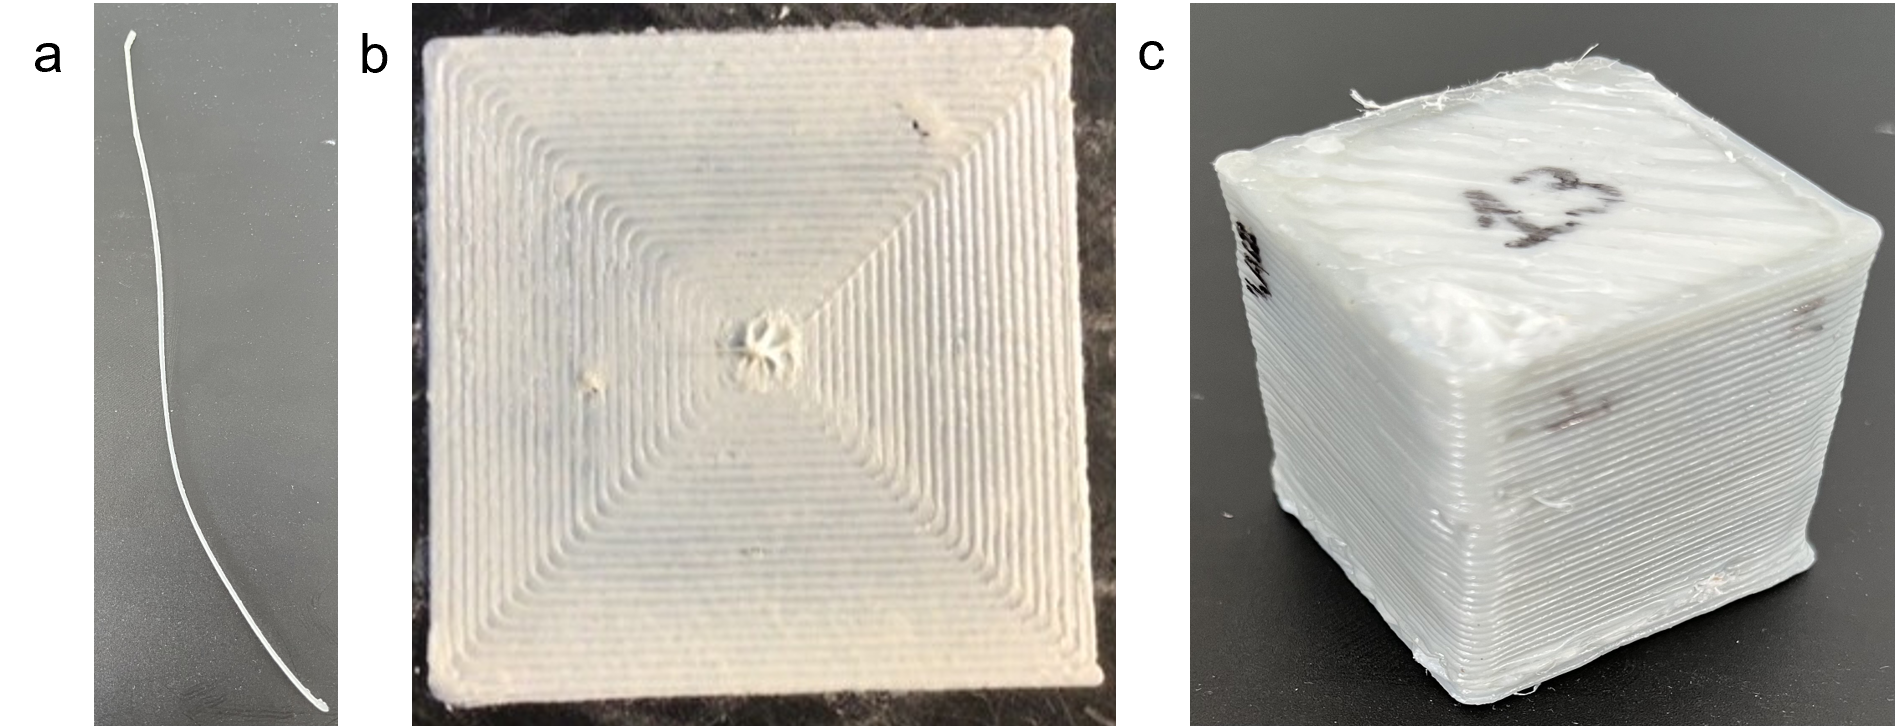
\includegraphics{figures/Figure_9_geometries.png}

}

\caption{\label{fig-geometries}Images of the resulting geometries a)
line, b) plane, c) cube}

\end{figure}

Afterwards, these parameters were used as initial guesses for plane
geometry, which achieved the desired fitness in the first iteration.
Similarly, cubes were printed using the plane ideal parameter as the
initial guess, and optimal parameters, were found in the first
iteration. The results showed a significant decrease in printing speed,
as the geometry complexity increased. Moreover, the cube geometry
required a higher extrusion multiplier to fill gaps and overcome
under-extrusion problems. The optimization of parameters for the three
geometries took approximately 10h reducing the experimental time,
compared to conventional methods. According to @oberloier2022, this
experimentation time can be reduced by 97\%. Indeed, the effectiveness
of PSO in finding global optimum parameters is high, especially in cases
with a large or complex design space {[}@saad2019a; @selvam2020{]}.

Additionally, PSO converge to optimum solutions with fewer iterations
than DoE methods {[}@zhang2015{]}. Combining PSO with other
meta-heuristic methods has demostrated higher ability to predict and
optimize parameters (e.g.~minimize surface
roughness{[}@shirmohammadi2021{]}, compressive strength and porosity of
scaffolds {[}@asadi-eydivand2016{]},and mechanical
properties{[}@raju2019{]}). However, DoE methods are still widely used
as they provide insight into the effects of individual design parameters
and their interactions while the ability to find interaction between the
variables is not possible using PSO. In the beginning of optimization
experiments, the understanding the process technique and function
settings might be complex. The methodology used in this study, however,
was easy to implement and the software used was free, open source, and
user-friendly, which reduced the initial difficulty. Therefore, PSO was
demonstrated to be an effective and highly accurate prediction technique
for finding the initial optimum parameters for rPET90//rHDPE10 material
for FGF/FPF.

Based on the result, it is evident that the optimal parameters for
printing may vary depending on the object and each parameter has its own
variation. One possible hypothesis is that the geometry of the object
could influence the assignment of parameters and this effect might be
more noticeable in large printings, yet further investigation is
required to confirm this hypothesis. There are several physical
mechanisms at play that are expected to alter the optimal printing
parameters based on size and geometry of the object. For example, the
cooling time and temperature history of a voxel will depend on the
geometry of the printed object {[}@cleeman2022{]}. Thus, to maintain a
consisten thermal history the printing parameters must be ajusted as the
geometry changes. This thermal history can also have more subtle
effects, such asimpacting the degree of crystallization even in the case
of PLA {[}@wijnen2018{]}.

In addition, the effects of material extrusion are magnified with scale,
including the impact of thermal expansion and contraction. Small changes
in contraction during cooling may cause acceptable distortions for small
prints, but these are magnified for larger prints (e.g.~causing
deformation and in the worst cases delamination or loss of bed
adhesion){[}@shah2019{]}. Although, @roschli2019 showed the obstacles
and possible solutions of the large-scale AM according to the way the
parts are designed the incidence of the geometry in the printing
parameters needs far more detailed future studies. Specifically better
models for mapping 3-D printing parameter optimization of small printed
objects to large-volume objects are needed.

\hypertarget{tbl-table3}{}
\begin{table}
\caption{\label{tbl-table3}Ideal printing parameters for fused granule fabrication of waste PET and
HDPE blend made from shredded whole plastic water bottles }\tabularnewline

\centering\begingroup\fontsize{10}{12}\selectfont

\begin{tabular}[t]{llllll}
\toprule
Variable & Line value & Planes value & Cube value & Δ & Units\\
\midrule
\cellcolor{gray!6}{T1} & \cellcolor{gray!6}{258} & \cellcolor{gray!6}{263} & \cellcolor{gray!6}{264} & \cellcolor{gray!6}{6 ±3.2} & \cellcolor{gray!6}{°C}\\
Tb & 86 & 82 & 84 & 4±2 & °C\\
\cellcolor{gray!6}{Ps} & \cellcolor{gray!6}{21} & \cellcolor{gray!6}{14} & \cellcolor{gray!6}{10} & \cellcolor{gray!6}{11±5.6} & \cellcolor{gray!6}{mm/s}\\
E & 1.07 & 0.87 & 1.32 & 0.5±0.3 & -\\
\bottomrule
\end{tabular}
\endgroup{}
\end{table}

\hypertarget{functional-object-print}{%
\subsection{Functional object print}\label{functional-object-print}}

The final parameters for print the case study product were determined
based on the ideal paraeters found for the cube geometry.However, the
print speed was ajusted to decrease the printing time and prevent
delamination. This adjustment was made in accordance with the PSO
results, which indicated that the material can be printed at a speed
range of 10 to 20 \(mm/s\). Increasing the printing speed reduces the
cooling time between the layers,thereby minimizing the risk of
delamination {[}@roschli2019{]}, This is particularly important for
larger objects, as delamination tends to be more pronounced in such
cases.

The Gigabot X successfully produced a piece of furniture from
multi-material recycled water bottles that included mixing HDPE and PET
as shown in Figure~\ref{fig-child} a.

The printing quality is acceptable as a prototype, proving the machine's
capacity to print large-scale functional objects. The chair was able to
comfortably hold a child with a mass of 20 kg, as shown in
Figure~\ref{fig-child} f.~However, further evaluation is needed for the
material used in the printing process. the printed object showed weak
bond strength between the adjacent layers resulting in delamination, as
seen in Figure~\ref{fig-child} b . This could be attributed to the
difference in chemical properties of the materials, their immiscibility
{[}@chu2022; @william2021{]}, high crystallinity {[}@verma2023{]} and
the large volume of the object as delamination issues were more
prominent during the printing of the chair compared to the parameters
optimization process. The delamination observed in larger objects can be
attributed to the rapid cooling of the layers before the material is
once again deposited. This is in contrast to cube printing, where the
smaller surface area allows better layer adhesion before complete
cooling. Even popular 3-D printing materials like PLA can be affected by
this issue, as observed from the print surface {[}@wijnen2018{]}. To
address the delamination problem and improve material properties, the
addition of agents that reduce could be benificial {[}@kramer1994;
@dai1997; @inoya2012{]}. This can enhance interfacial bonds through
polymer modification {[}@gao2021{]} and viscosity reduction
{[}@ko2019{]}. Additionally,we observed printing warping problems
(Figure~\ref{fig-child} c), which are likely caused by the high
crystallization rates of HDPE {[}@schirmeister2019{]}. we tested the use
of Magigoo adhesive (Thougth3D Ltd., Paola, Malta) and the addition of a
brim to improve bed adhesion, yet these solutions did not completely
resolve the problem. A previous study showed that the use of a building
plate made of thermoplastic elastomer SEBS allowed the adhesion of the
plastic and facilitated easy detachment of the printed object without
any breakage or damage {[}@schirmeister2019.This suggests a potencial
solution that should be further evaluated in future work. Another
visible issue present in the close angles of the printed object was the
shrinkage (Figure~\ref{fig-child} d) which occurs during solidification
and particularly upon polymer crystallization. Moreover, it is
well-known that PET has hygroscopic tendencies and easily absorbs
moisture from the temperature, which makes it difficult to extrude
{[}@bustosseibert2022{]}. As result, it is likely to break down in the
presence of water, lowering the quality of the print. Prior to printing
the chair some samples exhibited brittle behavior and void formation
therefore, the material was consistently dried and the hopper was kept
closed to prevent moisture from entering the environment.These measures
helped to ensure a more suitable material for printing.Additionally,
there are visible vibration and ringing problems (Figure~\ref{fig-child}
e) caused by the machine upgrades.Both acceleration and jerk (the
maximum value of instantaneous speed change) require finer tuning to
resolve these issues.

\begin{figure}

{\centering 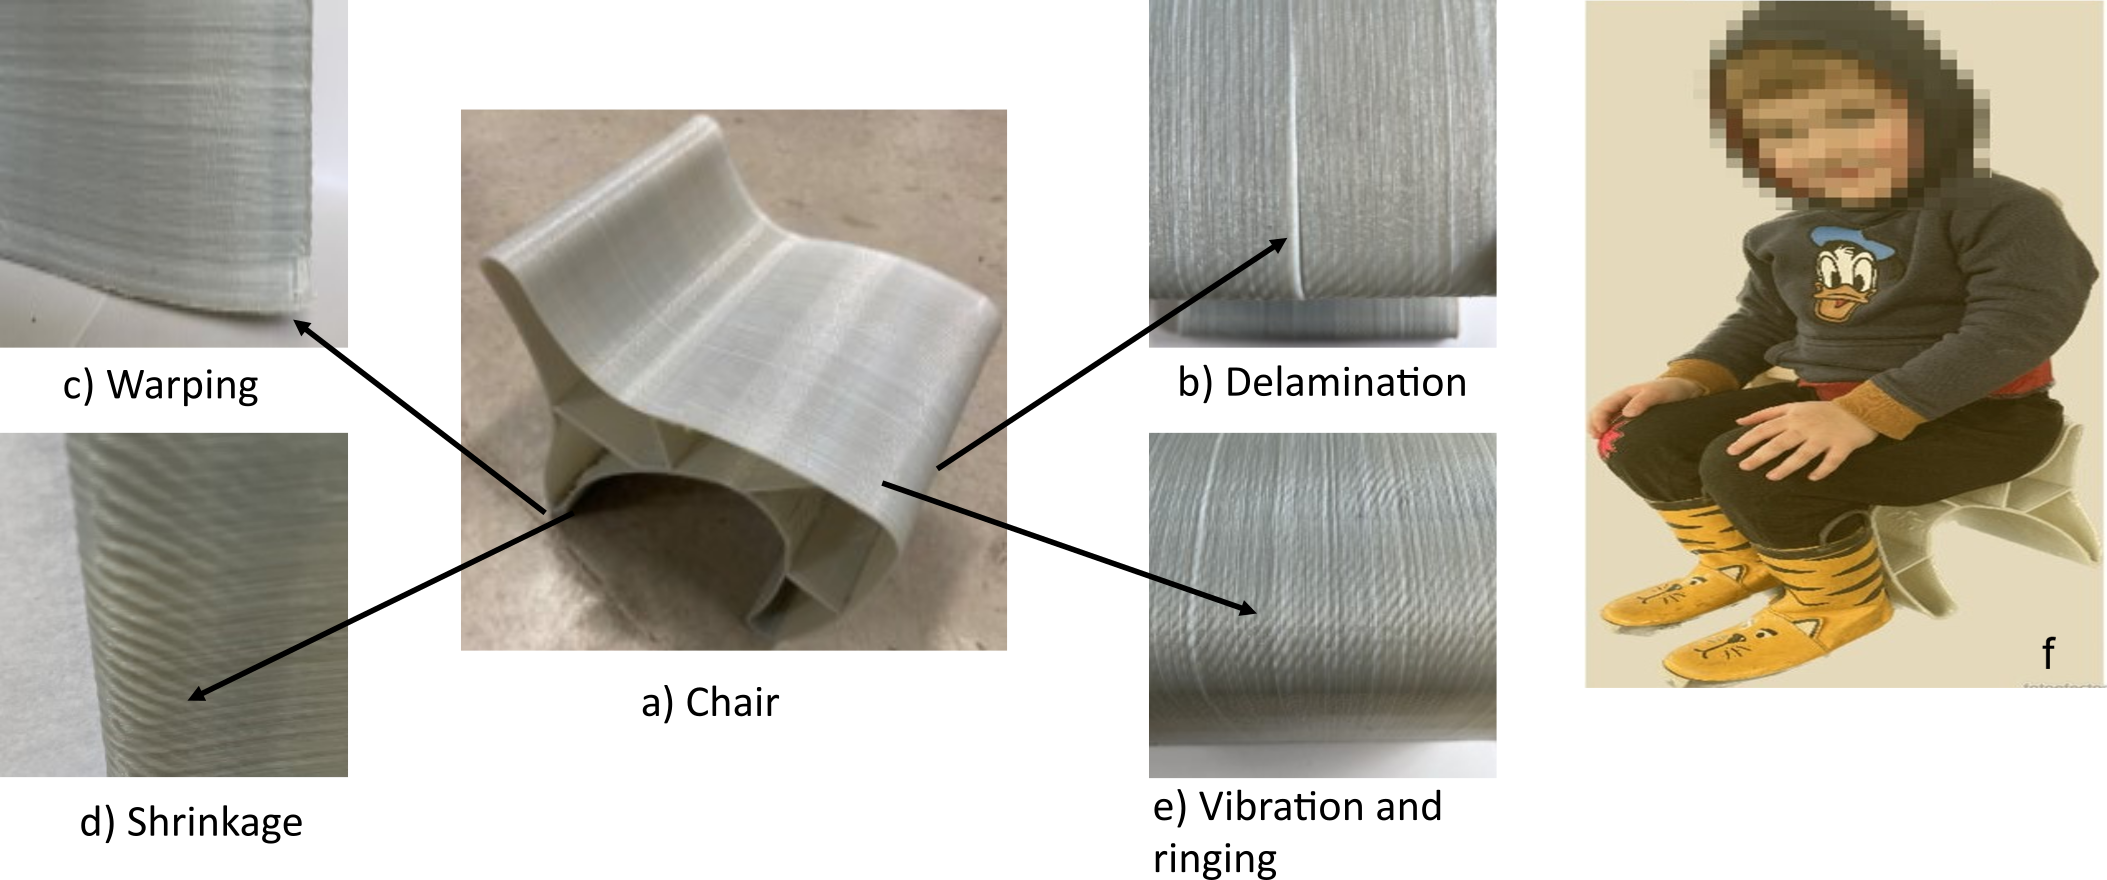
\includegraphics{figures/Figure6.png}

}

\caption{\label{fig-child}Finished children's chair and printing issues}

\end{figure}

\hypertarget{cost-and-environmental-impact}{%
\subsubsection{Cost and environmental
impact}\label{cost-and-environmental-impact}}

The printing process took 10 hours and the printed object weighs 840
grams. Due to the found optimized speed being low, the printing rate (
grams per hour) is low considering the machine that pellet printers have
a typical throughput of 220 g to 9 kg per hour. To improve the printing
time, upgrading the the extruder motor to a more powerful would be
benefitial. Besides, the energy required for 10 hours of 3-D printing
was found to be 6 kW-hr resulting in a production cost of
\textasciitilde1.2 € in function of the electricity cost in France, and
does not include the material cost, as the bottles used were obtained
from post-consumer waste. When labor costs are not included, the price
was significant reduced (\textasciitilde88\%) compared to the low-cost
options available in the market.

The economics of fabricating the case study product remained competitive
even when using recycled plastic pellets or shreds, which are avalable
on the market for prices ranging from 1-10 €/kg. However, it is
important to note that labor, maintenance, and machine devaluation were
not considered in the final price. These factors should be considered in
future work to ensure a comprehensive economic evaluation.

Regarding the environmental impact, this study does not evaluate the
entire life cycle of the printed object. However, various scientific
studies have already shown the feasibility of distributed recycling
{[}@santander2020; @kerdlap2022{]}. A comparison between conventional
and distributed manufacturing in terms of energy consumption and
emissions has been conducted {[}@Kreiger2013{]}. Other studies have
examined the environmental performance of AM {[}@garcia2018;
@colorado2020a{]} and the appearance of DRAM as a source of raw material
for diverse 3-D printers coming from post-consumer plastic waste in the
form of either filament {[}@hart2018; @pakkanen2017; @mohammed2017a;
@mikula2021{]} or granules {[}@alexandre2020{]}.

Additionally, @caceres-mendoza2023 have developed a comprehensive life
cycle assessment of a DRAM system focusing on the production of PLA
filament, comparing virgin and recycled materials. The findings of their
environmental analysis revealed a analysis revealed a reduction of
approximately 97\% in the production impacts, including climate change,
fossil depletion, water depletion, and potential eutrophication, when
using recycled filament as opposed to virgin filament. It is important
to note that these results are subject to the energy supply and might
vary depending on the geographical location.

\hypertarget{conclusion-and-future-work}{%
\section{Conclusion and future work}\label{conclusion-and-future-work}}

This study examined the feasibility of using mixed post-consumer waste
as a feedstock material for direct 3-D printing without the need of
compatibilization. The results demostrated the potential of mixing solid
waste plastics (PET/HDPE) to be used as feedstock material, as evidenced
by successfully printing a water bottle using two incompatible polymers
from the cap and body of the bottle. Additionally, the results found
that a large-scale FGF 3-D printer was capable of producing
cost-effective functional object using these mixed waste PET/HDPE
plastics. However, further research is necessary to analyze the
mechanical properties of the material and explore the use of
compatibilizers that can enhance the interphase tension between plastics
and reduce their crystallinity. These measures could potentially improve
and enhance the properties of both the material and the 3-D printed
parts.

These considerations become increasingly important as the size of the
3-D printed part increases. The improvement of the material science of
this approach can also offer an opportunity to improve the quality of
the printing time, reduce energy consumption of the machine, and improve
the economic viability of DRAM using mixed plastic waste.

In addition, future work could assess the different combinations or
blends of commodity plastics with or without the use of compatibilizers,
to determine their printability. This investigation could lead ti the
elimination of the selection/sorting process. In the same way, the
development of a methodology that ensure process reproducibility, even
in areas with limited infrastructure opens up the potential for plastic
revalorization using DRAM.

\hypertarget{declaration-of-competing}{%
\section*{Declaration of competing}\label{declaration-of-competing}}
\addcontentsline{toc}{section}{Declaration of competing}

The authors declare that they have no known competing financial
interests or personal relationships that could have appeared to
influence the work reported in this paper.

\hypertarget{acknowledgments}{%
\section*{Acknowledgments}\label{acknowledgments}}
\addcontentsline{toc}{section}{Acknowledgments}

This project has received funding from the European Union's Horizon 2020
research and innovation program under grant agreement No 869952. The
authors thank the LUE program for the financing of the thesis, the
Lorraine Fab Living lab platform and the Thompson endowment.

\newpage

\hypertarget{references}{%
\section*{References}\label{references}}
\addcontentsline{toc}{section}{References}

\setstretch{1.1}



\end{document}
